\documentclass[twoside,11pt]{article}

% Any additional packages needed should be included after jmlr2e.
% Note that jmlr2e.sty includes epsfig, amssymb, natbib and graphicx,
% and defines many common macros, such as 'proof' and 'example'.
%
% It also sets the bibliographystyle to plainnat; for more information on
% natbib citation styles, see the natbib documentation, a copy of which
% is archived at http://www.jmlr.org/format/natbib.pdf

\usepackage{jmlr2e}


% Definitions of handy macros can go here


\def\argmax{\mathop{\rm argmax}}
\def\argmin{\mathop{\rm argmin}}
\def\arginf{\mathop{\rm arginf}}
\def\Cov{\mathop{\rm Cov}}
\def\Var{\mathop{\rm Var}}
\def\sign{\mathop{\rm sign}}
\def\Sgn{\mathop{\rm Sgn}}
\def\arg{\mathop{\rm arg}}
\def\err{\mathop{\rm Err}}
\def\E{\mathop{\rm E}}
\def\diag{\mathop{\rm diag}}

\newcommand {\bfphi} {\mbox{\boldmath $\phi$}}
\newcommand {\bfbeta} {\mbox{\boldmath $\beta$}}
\newcommand {\bfalpha} {\mbox{\boldmath $\alpha$}}
\newcommand {\bfdelta} {\mbox{\boldmath $\delta$}}
\newcommand {\bfsigma} {\mbox{\boldmath $\sigma$}}
\newcommand {\bfSigma} {\mbox{\boldmath $\Sigma$}}
\newcommand {\bftheta} {\mbox{\boldmath $\theta$}}
\newcommand {\bfgamma} {\mbox{\boldmath $\gamma$}}
\newcommand {\bflambda} {\mbox{\boldmath $\lambda$}}
\newcommand {\bfepsilon} {\mbox{\boldmath $\epsilon$}}
\newcommand {\bfOmega} {\mbox{\boldmath $\Omega$}}

\def\bx{\mathop{\bf x}}
\def\bX{\mathop{\bf X}}
\def\bF{\mathop{\bf F}}
\def\bK{\mathop{\bf K}}
\def\bL{\mathop{\bf L}}
\def\by{\mathop{\bf y}}
\def\bY{\mathop{\bf Y}}
\def\bz{\mathop{\bf z}}
\def\bZ{\mathop{\bf Z}}
\def\bs{\mathop{\bf s}}
\def\bg{\mathop{\bf g}}
\def\bB{\mathop{\bf B}}
\def\bA{\mathop{\bf A}}
\def\bC{\mathop{\bf C}}
\def\bG{\mathop{\bf G}}
\def\bW{\mathop{\bf W}}
\def\be{\mathop{\bf e}}
\def\bI{\mathop{\bf I}}
\def\bH{\mathop{\bf H}}
\def\bM{\mathop{\bf M}}
\def\bT{\mathop{\bf T}}
\def\bu{\mathop{\bf u}}
\def\bv{\mathop{\bf v}}
\def\bU{\mathop{\bf U}}
\def\bt{\mathop{\bf t}}
\def\bz{\mathop{\bf z}}

\def\trans{^{ \mathrm{\scriptscriptstyle T} }}
\bibpunct[; ]{(}{)}{,}{a}{}{;}

\def\be{\begin{eqnarray}}
\def\bse{\begin{eqnarray*}}
\def\ee{\end{eqnarray}}
\def\ese{\end{eqnarray*}}

\def\wh{\widehat}
\def\wt{\widetilde}
\def\ol{\overline}

\newcommand{\dataset}{{\cal D}}
\newcommand{\fracpartial}[2]{\frac{\partial #1}{\partial  #2}}

% Heading arguments are {volume}{year}{pages}{submitted}{published}{author-full-names}

\jmlrheading{19}{2018}{1-21}{6/17}{12/18}{17-370}{Yixin Fang, Jinfeng Xu and Lei Yang}

% Short headings should be running head and authors last names

\ShortHeadings{Online Bootstrap for SGD}{Yixin Fang, Jinfeng Xu and Lei Yang}
\firstpageno{1}

\begin{document}

\title{Online Bootstrap Confidence Intervals for the Stochastic Gradient Descent Estimator}

\author{\name Yixin Fang \email yixin.fang@njit.edu \\
       \addr Department of Mathematical Sciences\\
       New Jersey Institute of Technology
       \AND
       \name Jinfeng Xu \email xujf@hku.hk \\
       \addr Department of Statistics and Actuarial Science \\
       The University of Hong Kong
       \AND
       \name Lei Yang \email ly888@nyu.edu \\
       \addr Department of Population Health \\
       New York University School of Medicine
       }

\editor{Gabor Lugosi}

\maketitle

\begin{abstract}%   <- trailing '%' for backward compatibility of .sty file
In many applications involving large dataset or online learning, stochastic gradient descent (SGD) is a scalable algorithm to compute parameter estimates and has gained increasing popularity due to its numerical convenience and memory efficiency. While the asymptotic properties of SGD-based estimators have been well established, statistical inference such as interval estimation remains much unexplored.  The classical bootstrap is not directly applicable if the data are not stored in memory. The plug-in method is not applicable when there is no explicit formula for the covariance matrix of the estimator. In this paper, we propose an online bootstrap procedure for the estimation of confidence intervals, which, upon the arrival of each observation, updates the SGD estimate as well as a number of randomly perturbed SGD estimates. The proposed method is easy to implement in practice. We establish its theoretical properties for a general class of models that includes linear regressions, generalized linear models, M-estimators and quantile regressions as special cases. The finite-sample performance and numerical utility is evaluated by simulation studies and real data applications.
\end{abstract}

\begin{keywords}
Bootstrap, Interval estimation, Generalized linear models, Large datasets, M-estimators, Quantile regression, Resampling methods, Stochastic gradient descent
\end{keywords}

\section{Introduction}
Big datasets arise frequently in clinical, epidemiological, financial and sociological studies. In such applications, many classical optimization methods for parameter estimation such as Fisher scoring, the EM algorithm or iterated reweighted least squares \citep{Hastie09,Nelder72} do not scale well and are computationally less attractive. Due to its computational and memory efficiency, stochastic gradient descent \citep{Robbins51}[SGD] is a scalable algorithm for parameter estimation and has recently drawn a great deal of attention. Unlike other classical methods that evaluate the objective function involving the entire dataset, the SGD method calculates the gradient of the objective function using only one data point at a time and recursively updates the parameter estimate. This is also numerically appealing and particularly useful in online updating settings such as streaming data where it may not even be feasible to store the entire dataset in memory. \citet{Wang16} gave a nice review on recent achievements of applying the SGD method to big data and streaming data.

The asymptotic properties of SGD estimators such as consistency and asymptotic normality have been well established; see, for example, \cite{Ruppert88} and \cite{Polyak92}. However, statistical inference such as confidence interval estimation for SGD estimators has remained largely unexplored. Traditional interval estimation procedures such as the plug-in procedure and the bootstrap are often numerically difficult in the presence of big datasets. The bootstrap repeatedly draws samples from the entire dataset. The plug-in procedure requires an explicit variance-covariance formula.  Since the classical bootstrap is not directly applicable if the data are not stored in memory, using the deal from the weighted bootstrap \citep{Rubin81}, we propose an online bootstrap procedure for the estimation of confidence intervals.

There are only a few papers considering the statistical inference of the SGD method. \cite{Chen16} proposed a method called the batch-mean procedure. Although computationally efficient and theoretically sound, the batch-means procedure substantially underestimates the variance of the SGD estimator in finite-sample studies, because of the correlations between the batch means. \cite{Li17} presented a new method for statistical inference in M-estimation problems, based on SGD estimators with a fixed step size. However, this method is limited to M-estimation and fixed step size. \cite{Su18} proposed a new method called HiGrad, short for Hierarchical Incremental GRAdient Descent, which estimates model parameters in an online fashion and provides a confidence interval for the true population value. This method is also computationally efficient and theoretically sound, but it is not applicable to vanilla SGD estimators.

In this paper, we propose an online bootstrap resampling procedure to approximate the distribution of a SGD estimator in a general class of models that includes linear regressions, generalized linear models, M-estimators and quantile regressions as special cases. Our proposal, justified by asymptotic theories, provides a simple way to estimate the covariance matrix and confidence regions. Through numerical experiments, we verify the ability of this procedure to give accurate inference for big datasets.

The rest of the article is organized as follows. In Section 2,  we introduce the proposed online bootstrap procedure for constructing confidence regions. In Section 3, we theoretically justify the validity of our proposal for a general class of models, along with some special cases. In Section 4, we demonstrate the performance of the proposed procedures in finite samples via simulation studies and three real data applications. Some concluding remarks are given in Section 5 and all the technical proofs are relegated to the Appendix.




\section{The proposed resampling procedure}

Parameter estimation by optimizing an objective function is often encountered in statistical practice. Consider the general situation where the optimal model parameter $\theta_0\in \mathcal{R}^p$ is defined to be the minimizer of the expected loss function,
\begin{eqnarray}\label{theta-0}
{\theta}_0=\argmin_{\theta\in\Theta}\left\{L(\theta)\triangleq \mathbb{E}[\ell(\theta; Z)]\right\},
\end{eqnarray}
where $\ell(\theta; z)$ is some loss function and $Z$ denotes one single observation and $\Theta$ is the domain on which the loss function is defined, which is assumed to be open. Suppose that the data consist of independent and identically distributed (i.i.d.) copies of $Z$,  denoted by $\mathcal{D}_N=\{Z_1, \dots, Z_N\}$. Under mild conditions, $\theta_0$ can be consistently estimated by
\begin{eqnarray}\label{est-regular}
\wt{\theta}_N=\argmin_{\theta\in\Theta}\left\{\frac{1}{N}\sum_{i=1}^{N}\ell(\theta; Z_i)\right\}.
\end{eqnarray}
However, the minimization problem (\ref{est-regular}) for large-scale datasets pose numerical challenges. Furthermore, for applications such as online data where each sample arrives sequentially (e.g., search queries or transactional data), it may not be necessary or feasible to store the entire dataset, leaving alone evaluating the minimand in (\ref{est-regular}).

As a stochastic approximation method \citep{Robbins51}, stochastic gradient descent is a scalable algorithm for parameter estimation with large-scale data. Given an initial estimate $\wh{\theta}_0$, the SGD method recursively updates the estimate upon the arrival of each data point $Z_n$, $n=1, 2, \dots, N$,
\begin{eqnarray}\label{SGD}
\wh{\theta}_n=\wh{\theta}_{n-1}-\gamma_n\nabla \ell(\wh{\theta}_{n-1}; Z_n),
\end{eqnarray}
where the learning rates are $\gamma_n=\gamma_1 n^{-\alpha}$ with $\gamma_1>0$ and $\alpha\in (0.5, 1)$. As suggested by \cite{Ruppert88} and \cite{Polyak92}, we consider the averaging estimate,
\begin{eqnarray}\label{SGD-avg}
\ol{\theta}_n=\frac{1}{n}\sum_{i=1}^n\wh{\theta}_i,
\end{eqnarray}
which can also be recursively updated given that $\ol{\theta}_n=(n-1)\ol{\theta}_{n-1}/n+\wh{\theta}_n/n$.

In order to conduct statistical inference with the averaging SGD estimator $\ol{\theta}_n$ at any stage, we propose an online bootstrap resampling procedure, which recursively updates the SGD estimate as well as a large number of randomly perturbed SGD estimates, upon the arrival of each data point. Specifically, let $\mathcal{W} = \{W_i, i = 1, \dots, N\}$ be a set of i.i.d. non-negative random variables with mean and variance equal to one. In parallel with (\ref{SGD}) and (\ref{SGD-avg}), with $\wh{\theta}^*_0\equiv \wh{\theta}_0$, upon observing data point $Z_n$, we recursively updates randomly perturbed SGD estimates,
\begin{eqnarray}
\wh{\theta}^*_n&=&\wh{\theta}^*_{n-1}-\gamma_nW_n\nabla \ell(\wh{\theta}^*_{n-1}; Z_n),\label{SGD-wt}\\
\ol{\theta}^*_n&=&\frac{1}{n}\sum_{i=1}^n\wh{\theta}^*_i.\label{SGD-avg-wt}
\end{eqnarray}

We will show that $\sqrt{n}(\ol{\theta}_n-{\theta}_0)$ and $\sqrt{n}(\ol{\theta}^*_n-\ol{\theta}_n)$ converge in distribution to the same limiting distribution. In practice, these results allow us to estimate the distribution of $\sqrt{n}(\ol{\theta}_n-{\theta}_0)$ by generating a large number, say $B$, of random samples of $\mathcal{W}$. We obtain  $\ol{\theta}^{*,b}_n$ by sequentially updating perturbed SGD estimates for each sample, $b=1, \dots, B$,
\begin{eqnarray}
\wh{\theta}^{*,b}_n&=&\wh{\theta}^{*,b}_{n-1}-\gamma_nW_{n,b}\nabla \ell(\wh{\theta}^{*,b}_{n-1}; Z_n),\label{SGD-wt-b}\\
\ol{\theta}^{*,b}_n&=&\frac{1}{n}\sum_{i=1}^n\wh{\theta}^{*,b}_i,\label{SGD-avg-wt-b}
\end{eqnarray}
and then approximate the sampling distribution of $\ol{\theta}_n-\theta_0$ using the empirical distribution of $\{\ol{\theta}^{*,b}_n-\ol{\theta}_n, b = 1, ..., B\}$. Specifically, the covariance matrix of $\ol{\theta}_n$ can be estimated by the sample covariance matrix constructed from $\{\ol{\theta}^{*,b}_n,b = 1,...,B\}$. Estimating the distribution of $\sqrt{n}(\ol{\theta}_n-{\theta}_0)$ based on the distribution of $\sqrt{n}(\ol{\theta}^*_n-\ol{\theta}_n)|\mathcal{D}_n$ leads to the construction of $(1-\alpha)100\%$ confidence regions for $\theta_0$. The resulting inferential procedure retains the numerical simplicity of the SGD method, only using one pass over the data. The proposed inferential procedure scales well for datasets with millions of data points or more, and its theoretical validity can be justified for a general class models with mild regularity conditions as shown in the next section.




\section{Theoretical Results}

\subsection{Main theorems}

In this section, we derive some theoretical properties of $\ol{\theta}_n^*$, justifying that the conditional distribution of $\ol{\theta}_n^*-\ol{\theta}_n$ given data $\mathcal{D}_n=\{Z_1, Z_2, \dots, Z_n\}$ can approximate the sampling distribution of $\ol{\theta}_n-\theta_0$, under the following assumptions. Let $\|\cdot\|$ be the Euclidean norm for vectors and the operator norm for matrices. The proofs are presented in the Appendix.

\begin{enumerate}
	\item[(A1).] The objective function $L(\theta)$ is convex, continuously differentiable over $\theta\in \Theta$, and twice continuously differentiable at $\theta=\theta_0$, where $\theta_0$ is the unique minimizer of $L(\theta)$.

	\item[(A2).] The gradient of $L(\theta)$, $R(\theta)=\nabla L(\theta)$, is Lipschitz continuous with constant $L_1>0$; that is, for any  $\theta_1$ and $\theta_2$, $\|R(\theta_1)-R(\theta_2)\|\leq L_1\|\theta_1-\theta_2\|$.

	\item[(A3).] The Hessian matrix of $L(\theta)$, $S(\theta)=\nabla^2 L(\theta)$, exists and is positive definite at $\theta_0$ with $S_0=S(\theta_0)>0$ and is Lipschitz continuous at $\theta_0$ with constant $L_2>0$.

	\item[(A4).] Let $V_0=\mathbb{E}\left\{[\nabla \ell(\theta_0; Z)][\nabla \ell(\theta_0; Z)]\trans\right\}$.  Assume $\mathbb{E}\|\nabla \ell(\theta; Z)\|^2\leq C(1+\|\theta\|^2)$ for some $C$ and $\mathbb{E}\|\nabla \ell(\theta; Z)-\nabla \ell(\theta_0; Z)\|^2\leq \delta(\|\theta-\theta_0\|)$ for some $\delta(\cdot)$ with $\delta(x)\rightarrow 0$ as $x\rightarrow 0$.

	\item[(A5).] The learning rates are chosen as $\gamma_n=\gamma_1 n^{-\alpha}$ with $\gamma_1>0$ and $\alpha\in(0.5, 1)$.

	\item[(A6).] The perturbation variables, $W_1, W_2, \dots$, are non-negative i.i.d.~random variables satisfying that $\mathbb{E}(W_n)=\mbox{Var}(W_n)=1$.
\end{enumerate}

Following similar arguments in  \cite{Ruppert88} and \cite{Polyak92}, we can prove the asymptotic normality of the SGD estimator $\ol{\theta}_n$ under the above assumptions.

\begin{lemma}
	\label{normality-set1}
	If Assumptions A1-A5 are satisfied, then we have
	\begin{eqnarray}
	\sqrt{n}(\ol{\theta}_n-\theta_0) \Rightarrow \mathcal{N}\left(0, S_0^{-1}V_0S_0^{-1}\right), {\mbox \ in \ distribution,\ as\ } n \rightarrow \infty.
	\end{eqnarray}
\end{lemma}


From Lemma 1, we can conduct statistical inference based on $\ol{\theta}_n$ provided that we can estimate the covariance matrix $S_0^{-1}V_0S_0^{-1}$, or we can use some resampling procedure to approximate the sampling distribution of $\sqrt{n}(\ol{\theta}_n-\theta_0)$. We first derive the asymptotically linear representation of $\ol{\theta}_n^*$ for any perturbation variables that are i.i.d.~random variables satisfying that $\mathbb{E}(W_n)=1$.

\begin{theorem}
	\label{eq-th1}
	If Assumptions A1-A5 hold, and the perturbation variables, $W_1, W_2, \dots$, are non-negative i.i.d.~random variables satisfying that $\mathbb{E}(W_n)=1$, then we have,
	\begin{equation}
	\sqrt{n}(\ol{\theta}_n^*-\theta_0)=-\frac{1}{\sqrt{n}}S_0^{-1}\sum_{i=1}^n W_i \nabla \ell(\theta_0; Z_i)+o_p(1).
	\end{equation}
\end{theorem}


By Theorem 1, letting $W_n\equiv 1$, we derive the following representation for $\ol{\theta}_n$,
\begin{equation}\label{eq-W-equal-one}
\sqrt{n}(\ol{\theta}_n-\theta_0)=-\frac{1}{\sqrt{n}}S_0^{-1}\sum_{i=1}^n \nabla \ell(\theta_0; Z_i)+o_p(1).
\end{equation}
Then, considering the difference between (\ref{eq-th1}) and (\ref{eq-W-equal-one}), we have
\begin{equation}\label{eq-W-diff}
\sqrt{n}(\ol{\theta}_n^*-\theta_n)=-\frac{1}{\sqrt{n}}S_0^{-1}\sum_{i=1}^n (W_i-1) \nabla \ell(\theta_0; Z_i)+o_p(1).
\end{equation}


Let $\mathbb{P}^*$ and $\mathbb{E}^*$ denote the conditional probability and expectation given the data. Starting from (\ref{eq-W-diff}), we derive the following theorem.

\begin{theorem}
	\label{eq-th2}
	If Assumptions A1-A6 hold, then we have
	\begin{equation}
	\sup_{v\in\mathcal{R}^p}\left|\mathbb{P}^*\left(\sqrt{n}(\ol{\theta}^*_n-\ol{\theta}_n)\leq v\right)-\mathbb{P}\Big(\sqrt{n}(\ol{\theta}_n-\theta_0)\leq v\Big)\right| \rightarrow 0, {in\ probability. }
	\end{equation}
\end{theorem}



By Theorem 2, the Kolmogorow-Smirnov distance between $\sqrt{n}(\ol{\theta}^*_n-\ol{\theta}_n)$ and $\sqrt{n}(\ol{\theta}_n-\theta_0)$ converges to zero in probability. This validates our proposal of the perturbation-based resampling procedure for inference with SGD. In the next section, we consider some special cases where Assumptions A1-A4 are satisfied.


\subsection{Special cases}

\subsubsection{Cases where $\ell(\theta; Z)$ is twice differentiable}

If the loss function $\ell(\theta; Z)$ is twice differentiable, we can use the plug-in procedure to estimate the asymptotic covariance matrix of $\sqrt{N}(\ol{\theta}_N-\theta_0)$, $S_0^{-1}V_0S_0^{-1}$. That is, at the final step, $S_0$ and $V_0$ can be estimated respectively by
\begin{eqnarray}
\wh{S}_N=\frac{1}{N}\sum_{i=1}^N \nabla^2 \ell(\ol{\theta}_N; Z_i) \mbox{\ \  and \ } \wh{V}_N=\frac{1}{N}\sum_{i=1}^N [\nabla \ell(\ol{\theta}_N; Z_i)][\nabla \ell(\ol{\theta}_N; Z_i)]\trans. \label{plug-in-N}
\end{eqnarray}

However, the above final-step plug-in estimation is impractical for large-scale data or streaming data, because it requires that the whole dataset be stored. To overcome this problem, in practice we can estimate $S_0$ and $V_0$ recursively, for $n=1, 2, \dots$, using
\begin{eqnarray}
\wh{S}_n=\frac{1}{n}\sum_{i=1}^n \nabla^2 \ell(\ol{\theta}_i; Z_i) \mbox{\ \  and \ } \wh{V}_n = \frac{1}{n}\sum_{i=1}^n [\nabla \ell(\ol{\theta}_i; Z_i)][\nabla \ell(\ol{\theta}_i; Z_i)]\trans. \label{plug-in-R}
\end{eqnarray}

In the following, we examine two examples where $\ell(\theta; Z)$ is twice differentiable. Example 1 is linear regression, where the loss function $\ell(\theta; Z)$ is twice differentiable and the objective function $L(\theta)$ is strongly convex. Example 2 is logistic regression, where $\ell(\theta; Z)$ is twice differentiable but $L(\theta)$ is non-strongly convex. They are two examples of generalized linear models, one for quantitative outcome and the other for binary outcome. In these two examples, both the plug-in procedures and the proposed perturbation resampling procedure are robust to model mis-specification.

{\bf Example 1} (Linear regression) Suppose that $Z_n=(Y_n, X_n)$, $n=1, 2, \dots$, are i.i.d.~copies of $Z=(Y, X)$, where $Y$ is quantitative and $X$ is $p$-dim with $\mathbb{E}\|X\|^2<\infty$. Let
\begin{eqnarray}\label{eg-lm}
\theta_0=\arg\min_{\theta\in\mathcal{R}^p}\mathbb{E}\left(Y-X\trans\theta\right)^2,
\end{eqnarray}
where $\ell(\theta; Z)=(Y-X\trans\theta)^2$ is twice differentiable and $L(\theta)=\mathbb{E}\left(Y-X\trans\theta\right)^2$ is strongly convex. Moveover, $\nabla \ell(\theta; Z)=-2(Y-X\trans\theta)X$, $\nabla^2 \ell(\theta; Z)=2X\trans X$, $\nabla L(\theta)=2\mathbb{E}\{XX\trans\}\theta-2\mathbb{E}\{XY\}$, and $\nabla^2 L(\theta)=\mathbb{E}\{\nabla l(\theta; Z)\}=2\mathbb{E}\{XX\trans\}$. Letting $V_0=4\mathbb{E}\{(Y-X\trans\theta_0)^2XX\trans\}$ and $S_0=2\mathbb{E}\{XX\trans\}$, we can easily verify that Assumptions A1-A4 hold. The SGD and perturbed SGD updates for $\theta_0$, as defined in (\ref{SGD}) and (\ref{SGD-wt}) respectively, are
\begin{eqnarray}
\wh{\theta}_n&=&\wh{\theta}_{n-1}+2\gamma_n(Y_n-X_n\trans\wh{\theta}_{n-1})X_n,\label{eg1-sgd}\\
\wh{\theta}^*_n&=&\wh{\theta}^*_{n-1}+2\gamma_nW_n(Y_n-X_n\trans\wh{\theta}^*_{n-1})X_n.\label{eg1-sgd-rw}
\end{eqnarray}


{\bf Example 2} (Logistic regression) Suppose that $Z_n=(Y_n, X_n)$, $n=1, 2, \dots$, are i.i.d.~copies of $Z=(Y, X)$, where $Y=\pm 1$ and $X$ is $p$-dim with $\mathbb{E}\|X\|^2<\infty$. Let
\begin{eqnarray}\label{eg-logit}
\theta_0=\arg\min_{\theta\in\mathcal{R}^p}\mathbb{E}\left\{-\log\left(\frac{1}{1+\exp(-YX\trans\theta)}\right)\right\},
\end{eqnarray}
where $\ell(\theta; Z)=\log\left(1+\exp(-YX\trans\theta)\right)$ is twice differentiable and $L(\theta)=\mathbb{E}\{\ell(\theta; Z)\}$ is non-strongly convex. Moveover, $\nabla \ell(\theta; Z)=-\frac{1}{1+\exp(YX\trans\theta)}XY$, $\nabla^2 \ell(\theta; Z)=\frac{\exp(YX\trans\theta)}{[1+\exp(YX\trans\theta)]^2}XX\trans$, $\nabla L(\theta)=\mathbb{E}\left\{\nabla \ell(\theta; Z)\right\}$, and $\nabla^2 L(\theta)=\mathbb{E}\left\{\nabla^2 \ell(\theta; Z)\right\}$. Letting $V_0=\mathbb{E}\left\{\frac{1}{[1+\exp(YX\trans\theta)]^2}XX\trans\right\}$ and $S_0=\mathbb{E}\left\{\frac{\exp(YX\trans\theta)}{[1+\exp(YX\trans\theta)]^2}XX\trans\right\}$, we can easily verify that Assumptions A1-A4 hold. The SGD and perturbed SGD updates for $\theta_0$, as defined in (\ref{SGD}) and (\ref{SGD-wt}) respectively, are
\begin{eqnarray}
\wh{\theta}_n&=&\wh{\theta}_{n-1}+\gamma_nXY/[1+\exp(YX\trans\wh{\theta}_{n-1})],\label{eg2-sgd}\\
\wh{\theta}^*_n&=&\wh{\theta}^*_{n-1}+\gamma_nW_nXY/[1+\exp(YX\trans\wh{\theta}^*_{n-1})].\label{eg2-sgd-rw}
\end{eqnarray}

We conclude this subsection with some discussion on the strong convexity of objective function $L(\theta)$, which is strongly convex in Example 1 and is non-strongly convex in Example 2. If $L(\theta)$ is strongly convex, i.e.~there exists $\mu>0$ such that $L(\theta_1)\geq L(\theta_2)+\nabla L(\theta_2)\trans(\theta_1-\theta_2)+\mu\|\theta_1-\theta_2\|^2$ for any $\theta_1$ and $\theta_2$, \citet{Moulines11} derived a non-asymptotic bound for $(\mathbb{E}\|\ol{\theta}_n-\theta_0\|)^{1/2}$. The bound of $(\mathbb{E}\|\ol{\theta}_n-\theta_0\|)^{1/2}$ has several terms; the leading term is of order $O(n^{-1})$ and the next two leading terms have order $O(n^{\alpha-2})$ and $O(n^{-2\alpha})$, suggesting the setting $\alpha=2/3$ to make them equal. If $L(\theta)$ is non-strongly convex, \citet{Moulines11} derived a non-asymptotic bound for $\mathbb{E}[L(\wh{\theta}_n)-L(\theta_0)]$ and a non-asymptotic bound for $\mathbb{E}[L(\ol{\theta}_n)-L(\theta_0)]$. The bound of $\mathbb{E}[L(\wh{\theta}_n)-L(\theta_0)]$ is $O(\max\{n^{\alpha-1}, n^{-\alpha/2}\})$, also suggesting the setting $\alpha=2/3$ to achieve optimal rate $O(n^{-1/3})$. Using the Polyak-Ruppert averaging has allowed the bound of $\mathbb{E}[L(\ol{\theta}_n)-L(\theta_0)]$ to go from $O(\max\{n^{\alpha-1}, n^{-\alpha/2}\})$ to $O(n^{-\alpha})$. Therefore, we use $\alpha=2/3$ in the numerical results.

\subsubsection{Cases where $\ell(\theta; Z)$ is not twice-differentiable}

If the loss function $\ell(\theta; Z)$ is not twice-differentiable, neither the final-step plug-in estimation (\ref{plug-in-N}) nor the recursive plug-in estimation (\ref{plug-in-R}) is applicable. Fortunately, our proposal of scalable inference based on perturbation resampling is still applicable because it only depends on the first order derivative $\nabla \ell(\theta; Z)$. To understand this explicitly, consider the following example of robust regression via $\psi$-type M-estimator where the loss function may be not twice-differentiable.

{\bf Example 3} (Robust regression via $\psi$-type M-estimator) Suppose that $Z_n=(Y_n, X_n)$, $n=1, 2, \dots$, are i.i.d.~copies of $Z=(Y, X)$, where $Y$ is quantitative and $X$ is $p$-dim with $\mathbb{E}\|X\|^2<\infty$. Let $\rho(\cdot)$ be some convex function with $\rho(0)=0$ and we attempt to estimate
\begin{eqnarray}\label{eg-rr-rho}
\theta_0=\arg\min_{\theta\in\mathcal{R}^p}\mathbb{E}\rho\left(Y-X\trans\theta\right),
\end{eqnarray}
where $\ell(\theta; Z)=\rho(Y-X\trans\theta)$ and $L(\theta)=\mathbb{E}\rho\left(Y-X\trans\theta\right)$. This is robust regression via $\rho$-type M-estimator. If $\rho(\cdot)$ is differentiable with derivative $\dot{\rho}(\cdot)=\psi(\cdot)$, we can solve it via $\psi$-type M-estimator, solving the following equation,
\begin{eqnarray}\label{eg-rr-psi}
\mathbb{E}\left\{\psi\left(Y-X\trans\theta_0\right)X\right\}=0,
\end{eqnarray}
where $\nabla\ell(\theta; Z)=-\psi(Y-X\trans\theta)X$ and $\nabla L(\theta)=-\mathbb{E}\left\{\psi\left(Y-X\trans\theta\right)X\right\}$. Hence, the SGD and perturbed SGD updates for $\theta_0$, as defined in (\ref{SGD}) and (\ref{SGD-wt}) respectively, are
\begin{eqnarray}
\wh{\theta}_n&=&\wh{\theta}_{n-1}+\gamma_n\psi(Y_n-X_n\trans\wh{\theta}_{n-1})X_n,\label{SGD-M}\\
\wh{\theta}^*_n&=&\wh{\theta}^*_{n-1}+\gamma_nW_n\psi(Y_n-X_n\trans\wh{\theta}^*_{n-1})X_n.\label{SGD-M-wt}
\end{eqnarray}

If $\psi(\cdot)$ is not differentiable, neither the final-step plug-in estimation (\ref{plug-in-N}) nor the recursive plug-in estimation (\ref{plug-in-R}) is applicable. However, if the corresponding $\ell(\theta; Z)$ and $L(\theta)$ satisfy Assumptions A1-A4, the perturbation resampling procedure is applicable. Next we consider a special setting where the following Assumptions B1-B4 hold.

\begin{enumerate}
	\item[(B1).] Assume that $\rho(u)$ is a convex function on $\mathcal{R}$ with the right derivative being $\psi_+(u)$ and left derivative being $\psi_-(u)$. Let $\psi(u)$ be a function such that $\psi_-(u)\leq \psi(u) \leq \psi_+(u)$. There exists constant $C_1>0$ such that $|\psi(u)|\leq C_1(1+|u|)$.

	\item[(B2).] Let $\varepsilon_n=Y_n-X_n\trans\theta_0$. Assume that $(X_n,\varepsilon_n), n=1,2,...,$  are i.i.d.~copies of
	$(X,\varepsilon)$, with $\mathbb{E}\|X\|^4<\infty$ and $\mathbb{E}\|\varepsilon\|^2<\infty$. Let $V_0=\mathbb{E}\{\psi^2(\varepsilon)XX\trans\}>0$.

	\item[(B3).] Let $\phi(u|X)=\mathbb{E}\{\psi(u+\varepsilon)|X\}$. Assume that $\phi(0|X)=0$, $u\phi(u|X)>0$ for any $u\neq 0$, and $\phi(u|X)$ has a derivative at $u=0$ with $\dot{\phi}(0|X)\geq\sigma>0$ uniformly over $X$. Let $S_0=\mathbb{E}\{\dot{\phi}(0|X)XX\trans\}>0$.

	\item[(B4).] Assume that $\dot{\phi}(u|X)$ is uniformly Lipschitz at $u=0$. That is, there exist constants $C_2>0$ and $\delta>0$ such that $\left|\dot{\phi}(u|X)-\dot{\phi}(0|X)\right|\leq C_2|u|$ for $|u|\leq \delta$ uniformly over $X$.
	%
	%\item[(B4).] Let $\varphi(u)=\mathbb{E}\{\psi^2(u+\varepsilon)\}$. Assume that $\varphi(u)$ is finite for $u$ in a neighborhood of $u=0$ and is continuous at $u=0$. Let

\end{enumerate}


We derive the asymptotic properties of the $\psi$-type M-estimator as follows.

\begin{lemma}
	\label{normality-set2}
	If Assumptions B1-B4 and A5 are satisfied, then we have
	\begin{eqnarray}
	\sqrt{n}(\ol{\theta}_n-\theta_0) \Rightarrow \mathcal{N}\left(0, S_0^{-1}V_0S_0^{-1}\right), {\mbox \ in \ distribution,\ as\ } n \rightarrow \infty.
	\end{eqnarray}
\end{lemma}


\begin{theorem}
	\label{eq-th3}
	If Assumptions B1-B4 and A5-A6 are satisfied, then we have
	\begin{equation}
	\sqrt{n}(\ol{\theta}_n^*-\theta_0)=\frac{1}{\sqrt{n}}S_0^{-1}\sum_{i=1}^n W_i \psi(\varepsilon_i)X_i+o_p(1).
	\end{equation}
\end{theorem}


From Lemma 2 we see that the plug-in procedures are not applicable for estimating the asymptotic covariance matrix, because although they are applicable for estimating $V_0$, they are not applicable for estimating $S_0$, which involves $\dot{\phi}(0|X)$. Moreover, by Theorem 3, we can show that the Kolmogorow-Smirnov distance between $\sqrt{n}(\ol{\theta}^*_n-\ol{\theta}_n)$ and $\sqrt{n}(\ol{\theta}_n-\theta_0)$ converges to zero in probability, as stated in Theorem 2. This validates our proposal of the perturbation-based resampling procedure for robust regression. To further understand Assumptions B1-B4, we examine the following example of quantile regression, which is a special case of the above robust regression.

{\bf Example 4} (Quantile regression). Assume the $\tau$-quantile of $Y$ given $X$ is $X\trans\theta_0$, with
\begin{equation}
\theta_0=\arg\min_{\theta\in\mathcal{R}^p}\mathbb{E} \rho_{\tau}(Y-X\trans\theta),\label{eq-qr}
\end{equation}
where $\rho_\tau(u)=u(\tau-I(u<0))$ with a given $0<\tau<1$. Let $\varepsilon=Y-X\trans\theta_0$ and $\psi_{\tau}(u)=\tau-I(u<0)$. Thus $\mathbb{E}\{\psi_{\tau}(\varepsilon)|X\}=\tau-F_{\varepsilon}(0|X)=0$, where $F_{\varepsilon}(u|X)$ is the conditional distribution function of $\varepsilon$. Let $p_{\varepsilon}(u|X)$ be the conditional density function of $\varepsilon$. Note that $\phi(u|X)=\mathbb{E}\{\psi_{\tau}(u+\varepsilon)|X\}=\tau-F_{\varepsilon}(-u|X)$, $\dot{\phi}(0|X)=p_{\varepsilon}(0|X)$, $V_0=\mathbb{E}\{\psi^2_{\tau}(\varepsilon)XX\trans\}=\tau(1-\tau)\mathbb{E}\{XX\trans\}$ and $S_0=\mathbb{E}\{p_{\varepsilon}(0|X)XX\trans\}$. Therefore, we can easily verify that if $p_{\varepsilon}(0|X)$ is uniformly bounded away from 0 and $p_{\varepsilon}(u|X)$ is uniformly Lipschitz continuous at $u=0$, then Assumptions B1-B4 hold. Thus, the SGD and perturbed SGD updates for $\theta_0$, as defined in (\ref{SGD}) and (\ref{SGD-wt}) respectively, are
\begin{eqnarray}
\wh{\theta}_n&=&\wh{\theta}_{n-1}+\gamma_n\left\{\tau-I(Y_n-X_n\trans\wh{\theta}_{n-1}<0)\right\}X_n,\label{eg4-sgd}\\
\wh{\theta}^*_n&=&\wh{\theta}^*_{n-1}+\gamma_nW_n\left\{\tau-I(Y_n-X_n\trans\wh{\theta}^*_{n-1}<0)\right\}X_n,\label{eg4-sgd-rw}
\end{eqnarray}
and the asymptotic results stated in Lemma 2 and Theorem 3 follow directly.

\section{Numerical results}

\subsection{Simulation studies}

To assess the performance of the proposed online bootstrap resampling procedure (a.k.a. random weighting procedure; RW) for SGD estimators, we conduct simulation studies for those four examples discussed in Section 3. We compare the proposed procedure with the recursive plug-in procedure (RPI).

{\bf Setting 1} (Linear regression):  Consider linear regression (\ref{eg-lm}), where covariates $X^{(j)}$, $j=1, \dots, p$, and residual $\varepsilon=Y-X\trans\theta_0$, are independently generated from standard normal $N(0,1)$. Here $X^{(j)}$ indicates the $j$-th dimension of $X$. Let $\theta_0=(\mu{\bf 1}\trans_{q/2},-\mu{\bf 1}\trans_{q/2},{\bf 0}\trans_{p-q})\trans$ (same for the other three settings). Consider the corresponding SGD estimators (\ref{eg1-sgd}) and (\ref{eg1-sgd-rw}).

{\bf Setting 2} (Logistic regression): Consider logistic regression (\ref{eg-logit}), where covariates $X^{(j)}$ are independently from $N(0,1)$ and response $Y$ from Bernoulli distribution with $\mbox{logit}\{P(Y=1|X)\}=X\trans\theta_0$. Consider the corresponding SGD estimators (\ref{eg2-sgd}) and (\ref{eg2-sgd-rw}).

{\bf Setting 3} (LAD regression): Consider least absolute deviation (LAD) regression, which is a special case of robust regression (\ref{eg-rr-rho}) with $\rho(x)=|x|$ and quantile regression (\ref{eq-qr}) with $\tau=0.5$, where covariates $X^{(j)}$, $j=1, \dots, p$, are i.i.d.~with $N(0, 1)$ and residual $\varepsilon$, defined as $Y-X\trans\theta_0$, is independently from double exponential distribution $DE(0, 1)$. Consider the corresponding SGD estimators (\ref{eg4-sgd}) and (\ref{eg4-sgd-rw}) with $\tau=0.5$.

{\bf Setting 4} (LAD regression for data with outliers): Consider LAD regression for the data generated from Setting 1 but contaminated with $10\%$ outliers. The contaminated data are obtained by transforming the outcome variable in the data generated from Setting 1 using $Y \leftarrow Y +10$ if $|X^{(1)}|\geq 1.96$ and $|X^{(2)}|< 1.96$; and $Y \leftarrow Y -10$ if $|X^{(1)}|< 1.96$ and $|X^{(2)}|\geq 1.96$. In this setting, covariate vector $X$ and residual $\varepsilon=Y-X\trans\theta_0$ are not independent, but $\mbox{median}\{\varepsilon|X\}=0$. Consider the corresponding SGD estimators defined in (\ref{eg4-sgd}) and (\ref{eg4-sgd-rw}) with $\tau=0.5$.

For each simulation setting, we consider four scenarios, as described by $(N, p, q, \mu)$, where sample size $N=10,000$ or $20,000$, number of covariates $p=10$ or $20$, number of informative covariates $q=6$, and effect size $\mu=0.1$ or $0.2$. For each example, we repeat the data generation 1000 times. For each data repetition, we use $W_{nb}\sim{\rm exp}(1)$ as random weights and generate $B=200$ copies of random weights whenever a new data point is read. Then, for each data repetition, we obtain the SGD estimate (\ref{SGD-avg}), and apply the following procedures to construct $95\%$ confidence intervals: the proposed random weighting procedure to obtain $2.5\%$ and $97.5\%$ quantile (RW-Q), the proposed random weighting procedure to estimate its standard error (RW-$\sigma$) and then construct ``$\mbox{estimate}\pm 1.96\times\wh{\mbox{SE}}$", and the recursive plug-in procedures (RPI), if applicable, to estimate its standard error. We consider the learning rate $\alpha=2/3$. When we calculate the average SGD estimators (\ref{SGD-avg}) and (\ref{SGD-avg-wt}), the first 2000 and 4000 estimates are excluded for $N=10,000$ and $N=20,000$, respectively. We also obtain the empirical standard error based on 1000 repeated  SGD estimates, as a benchmark approximation to the true standard error.

The coverage probabilities of the 95\% confidence interval estimates are summarized in Table \ref{tab:sim1} for linear regression (Setting 1),  Table \ref{tab:sim2} for logistic regression (Setting 2) and Table \ref{tab:sim3} for LAD regression (Settings 3-4), respectively. We only report results corresponding to the first, fourth and seventh covariates (that is, $X^{(1)}$, $X^{(q/2+1)}$ and $X^{(q+1)}$). The plug-in procedures are not applicable for LAD regression in Settings 3-4.

From Tables \ref{tab:sim1} and \ref{tab:sim2}, we see that, for linear regression and logistic regression, the coverage probabilities using the RW-Q, RW-$\sigma$ and RPI are close to $95\%$. Therefore, the proposed random weighting procedures (both RW-Q and RW-$\sigma$) perform well for linear regression and logistic regression, and if we choose to use the plug-in procedure, which involves matrix inverse, we can use RPI. Since the point estimate is $\sum_{i=N_0+1}^N \wh{\theta}_i/(N-N_0)$, where $N_0$ is the number of excluded estimates and which involves a pass of SGD estimates, its standard error should also involve a pass of SGD estimates, instead of involving only the final-step estimate or the true parameter value. We can understand this clearer if we see the ``SE" column, where the standard errors from RW-$\sigma$ and RPI are close to the empirical standard error. Moveover, from Table  \ref{tab:sim3}, we see that, for LAD regression and for both Settings 3 and 4, the coverage probabilities using either of the two proposed random weighting procedures are close to $95\%$, and the standard errors using RW-$\sigma$ are close to the empirical standard errors.

\begin{table}[!h]
	\centering
	\caption{Coverage probabilities of 95\% confidence intervals for linear regression}
	\medskip
	\label{tab:sim1}
	\begin{tabular}{cccccccc}
		\hline
		$(N, p, q, \mu)$ & Method & \multicolumn{2}{c}{Dim 1} & \multicolumn{2}{c}{Dim $q/2+1$} & \multicolumn{2}{c}{Dim $q+1$}\\
		& & Cover& SE& Cover& SE & Cover& SE\\
		\hline
		\hline
		(10000,10,6,0.1) & RW-Q & 0.947& $-$& 0.946& $-$&0.950 & $-$\\
		& RW-$\sigma$ & 0.956&0.012 &0.950 & 0.012&0.959 & 0.012\\
		& RPI & 0.953&0.011 &0.946& 0.011&0.956& 0.011\\
		%		& FPI & 0.468& 0.004 &0.477& 0.004&0.462& 0.004\\
		%		& TPI & 0.797& 0.008&0.798 & 0.008&0.764& 0.008\\
		& Empirical & $-$& 0.011&$-$ & 0.011&$-$& 0.011\\
		\hline
		(10000,10,6,0.2)  & RW-Q & 0.947&$-$  &0.946&$-$ &0.950& $-$\\
		& RW-$\sigma$ & 0.956 & 0.012&0.950  & 0.012&0.959 &0.012\\
		& RPI & 0.953 &0.011 &0.946 & 0.011& 0.956& 0.011\\
		%		& FPI & 0.468& 0.004& 0.478& 0.004&0.462& 0.004\\
		%		& TPI & 0.797 & 0.008&0.798 & 0.008&0.764 &0.008\\
		& Empirical & $-$& 0.011&$-$ & 0.011&$-$& 0.011\\
		\hline
		(20000,20,6,0.1) & RW-Q & 0.939 & $-$&0.951 &$-$ &0.945&$-$\\
		& RW-$\sigma$ & 0.949 &0.008 &0.953 &0.008 &0.960&0.008\\
		& RPI & 0.956& 0.008& 0.948 & 0.008&0.957 &0.008\\
		%		& FPI & 0.473 & 0.003&0.447 & 0.003&0.444&0.003\\
		%		& TPI & 0.788&0.006 &0.778 &0.006& 0.783& 0.006\\
		& Empirical & $-$& 0.008&$-$ & 0.008&$-$& 0.008\\
		\hline
		(20000,20,6,0.2) & RW-Q & 0.939&$-$& 0.951&$-$& 0.945&$-$\\
		& RW-$\sigma$ &0.949 & 0.008&0.953 &0.008 &0.960&0.008\\
		& RPI & 0.956& 0.008& 0.948 & 0.008& 0.957& 0.008\\
		%		& FPI & 0.473 &0.003  &0.447& 0.003&0.444&0.003\\
		%		& TPI & 0.788&0.006 &0.778 & 0.006&0.783& 0.006\\
		& Empirical & $-$& 0.008&$-$ & 0.008&$-$& 0.008\\
		\hline
	\end{tabular}
\end{table}

\begin{table}[!h]
	\centering
	\caption{Coverage probabilities of 95\% confidence intervals for logistic regression}
	\medskip
	\label{tab:sim2}
	\begin{tabular}{cccccccc}
		\hline
		$(N, p, q, \mu)$ & Method & \multicolumn{2}{c}{Dim 1} & \multicolumn{2}{c}{Dim $q/2+1$} & \multicolumn{2}{c}{Dim $q+1$}\\
		& & Cover& SE& Cover& SE & Cover& SE\\
		\hline
		\hline
		(10000,10,6,0.1) & RW-Q & 0.950&$-$ &0.948 &$-$ &0.928&$-$\\
		& RW-$\sigma$ & 0.954&0.024 & 0.954&0.024 &0.948& 0.023\\
		& RPI & 0.954& 0.023& 0.952&0.023 &0.942 &0.023\\
		%		& FPI & 0.432& 0.008&0.450 & 0.008& 0.418& 0.008\\
		%		& TPI & 0.784&0.016 &0.790 &0.016 &0.828&0.017\\
		& Empirical & $-$& 0.022&$-$ & 0.022&$-$& 0.023\\
		\hline
		(10000,10,6,0.2) & RW-Q & 0.945&$-$ &0.945 &$-$ &0.944 &$-$\\
		& RW-$\sigma$ & 0.959& 0.025& 0.954& 0.025&0.954&0.024\\
		& RPI & 0.955&0.023 & 0.952& 0.023&0.948& 0.023\\
		%		& FPI &0.449 & 0.008&0.405 & 0.008&0.424&0.008\\
		%		& TPI & 0.785& 0.016 &0.814 & 0.017 &0.824& 0.017\\
		& Empirical & $-$& 0.023&$-$ & 0.023&$-$& 0.023\\
		\hline
		(20000,20,6,0.1) & RW-Q & 0.944&$-$ & 0.939&$-$ &0.934&$-$\\
		& RW-$\sigma$ & 0.951& 0.016&0.953 &0.016 &0.952& 0.016\\
		& RPI & 0.948&0.016 &0.953& 0.016&0.949& 0.016\\
		%		& FPI & 0.456& 0.005&0.446 &0.005 &0.451&0.005\\
		%		& TPI &0.777 & 0.012&0.813 & 0.012&0.796&0.012\\
		& Empirical & $-$& 0.016&$-$ & 0.016&$-$& 0.016\\
		\hline
		(20000,20,6,0.2) & RW-Q & 0.946&$-$ &0.941 & $-$&0.939&$-$\\
		& RW-$\sigma$ & 0.958& 0.017& 0.952 & 0.017&0.957 & 0.016\\
		& RPI &0.950 & 0.016&0.944 &0.016 &0.952 & 0.015\\
		%		& FPI &0.379 & 0.005&0.368&0.005  &0.377 &0.004\\
		%		& TPI & 0.830& 0.012 &0.836& 0.012&0.851 & 0.012\\
		& Empirical & $-$& 0.016&$-$ & 0.016&$-$& 0.016\\
		\hline
	\end{tabular}
\end{table}

\begin{table}[!h]
	\centering
	\caption{Coverage probabilities of 95\% confidence intervals for LAD regression}
	\medskip
	\label{tab:sim3}
	\begin{tabular}{cccccccc}
		\hline
		$(N, p, q, \mu)$ & Method & \multicolumn{2}{c}{Dim 1} & \multicolumn{2}{c}{Dim $q/2+1$} & \multicolumn{2}{c}{Dim $q+1$}\\
		& & Cover& SE& Cover& SE & Cover& SE\\
		\hline\hline
		\multicolumn{8}{c}{Simulation Setting 3}\\
		\hline
		(10000,10,6,0.1) & RW-Q & 0.965&$-$ &0.965&$-$ &0.969&$-$\\
		& RW-$\sigma$ & 0.969&0.029 &0.965& 0.029&0.965& 0.029\\
		& Empirical & $-$& 0.026&$-$ & 0.027&$-$& 0.026\\
		\hline
		(10000,10,6,0.2) &  RW-Q &0.972 & $-$&0.965 & $-$&0.967&$-$\\
		& RW-$\sigma$ & 0.973& 0.029& 0.966& 0.029&0.968 & 0.029\\
		& Empirical & $-$& 0.026&$-$ & 0.027&$-$& 0.026\\
		\hline
		(20000,20,6,0.1) & RW-Q & 0.970& $-$ &0.973 &$-$ &0.966 &$-$\\
		& RW-$\sigma$ & 0.966& 0.010&0.969 & 0.010&0.965& 0.010\\
		& Empirical & $-$& 0.009&$-$ & 0.009&$-$& 0.009\\
		\hline
		(20000,20,6,0.2)& RW-Q & 0.967& $-$&0.974& $-$ & 0.966&$-$\\
		& RW-$\sigma$ & 0.966& 0.010& 0.969& 0.010&0.969 & 0.010\\
		& Empirical & $-$& 0.009&$-$ & 0.009&$-$& 0.009\\
		\hline
		\multicolumn{8}{c}{Simulation Setting 4}\\
		\hline
		(10000,10,6,0.1) & RW-Q & 0.954&$-$ &0.971&$-$ &0.950 &$-$\\
		& RW-$\sigma$ & 0.958& 0.035&0.969&0.035 &0.960 &0.035\\
		&Empirical &$-$ &0.032&$-$ &0.031 &$-$ &0.033\\
		\hline
		(10000,10,6,0.2) &  RW-Q &0.960& $-$&0.966 &$-$&0.955&$-$ \\
		& RW-$\sigma$ & 0.958& 0.035& 0.966 & 0.035& 0.956& 0.035\\
		&Empirical &$-$ &0.032&$-$ &0.031 &$-$ &0.033\\
		\hline
		(20000,20,6,0.1) &  RW-Q & 0.948&$-$&0.953 &$-$ &0.965&$-$\\
		& RW-$\sigma$ &0.963&0.047 &0.958 & 0.047& 0.964& 0.047\\
		&Empirical &$-$ &0.043&$-$ &0.045 &$-$ &0.044\\
		\hline
		(20000,20,6,0.2) &  RW-Q & 0.944&$-$& 0.957 & $-$&0.961& $-$\\
		& RW-$\sigma$ &0.961& 0.047& 0.961& 0.047&0.961 & 0.047\\
		&Empirical &$-$ & 0.044&$-$ &0.045 &$-$ &0.044\\
		\hline
	\end{tabular}
\end{table}


\subsection{Real data applications}

In this section, we apply the proposed procedures to conduct inference for linear regression analysis for the individual household electric power consumption data (POWER) and logistic regression analysis for the skin segmentation dataset (SKIN) and gas sensors for the home Activity monitoring data (GAS). All the three datasets are publicly available on UCI machine learning repository.

The POWER dataset contains 2,075,259 observations and we fit a linear model to investigate how the time of a day influences the response variable ``sub-metering-1", the energy sub-metering No.~1, in watt-hour of active energy corresponding to kitchen. The observations with missing value are deleted, and the time of a day is divided into 8 categories, ``{\it Time 0-2}", ``{\it Time 3-5}", ..., and ``{\it Time 21-23}". The SKIN dataset contains 245,057 observations, out of which 50,859 is the skin samples and 194,198 is non-skin samples. We fit a logistic model to examine the relationship between the indicator of skin and three predictors, {\it B}, {\it G} and {\it R}. The GAS dataset contains 919,438 observations and we only use a subset containing 652,024 observations with response variable being either ``banana" or ``wine". We fit a logistic model to examine the association between the response variable and 11 explanatory variables, {\it Time}, {\it R1} to {\it R8}, {\it Temperature} and {\it Humidity}.

Although standard softwares such as SAS and R can fit linear and logistic regression to such datasets without difficulty, for the illustration purpose, we use the SGD as in Examples 1 and 2 to fit linear and logistic regression and use the proposed online boostrap procedure to construct confidence intervals. The point estimates and the 95\% confidence intervals of the coefficients are showed in Table \ref{tab:real-data}. From the left-top panel of Table \ref{tab:real-data}, we see that the electronic power consumption from kitchen is relatively high in the evening and night. From the left-bottom panel of Table \ref{tab:real-data}, we see that variable {\it B} is positively associated with the response while the other two variables {\it G} and {\it R} are negatively associated. From the right panel of Table \ref{tab:real-data}, we see that all the variables but {\it R4} are statistical significantly associated with the response. Furthermore, we display the histogram of $B=1000$ perturbation-based SGD estimates for each coefficient in Figures \ref{fig:fig-real-linear}-\ref{fig:fig-real-glm-2} for the POWER data, the SKIN data and the GAS data, respectively. The blue triangle in each figure indicates the corresponding point estimate the red triangles indicate 2.5 and 97.5 quantiles. From these figures, we see the the perturbation-based procedure can be used to approximate the sampling distribution of the corresponding SGD estimator, which might be skewed. For example, for the GAS data, the sampling distributions are very skewed, and therefore the proposed resampling procedure is able to display such skewness.

\begin{table}[!h]
	\centering
	\caption{Point estimates and 95\% confidence intervals for three real datasets; POWER data on the left-top panel, SKIN data on the left-bottom panel and GAS data on the right panel}
	\medskip
	\label{tab:real-data}
	\begin{tabular}{ccc|ccc}
		\hline
		Variable &Est. & 95\% CI & Variable &Est. & 95\% CI\\
		\hline\hline
		{\it Time 0-2} & $2.265$ & $(2.254,2.275)$ & {\it Time} & $-0.158$ & $(-0.178, -0.139)$\\
		{\it Time 3-5} & $2.045$ & $(2.040,2.049)$ & {\it R1} & $-0.202$ & $(-0.215, -0.190)$\\
		{\it Time 6-8} & $2.623$ & $(2.608,2.639)$ & {\it R2} & $0.176$ & $(0.160, 0.191)$ \\
		{\it Time 9-11} & $3.323$ & $(3.298,3.347)$ & {\it R3} & $-0.907$ & $(-0.932, -0.882)$\\
		{\it Time 12-14} & $3.445$ & $(3.420,3.470)$ & {\it R4} & $-0.007$ & $(-0.018, 0.004)$\\
		{\it Time 15-17} & $3.059$ & $(3.037,3.082)$ & {\it R5} & $-0.450$ & $(-0.467, -0.432)$\\
		{\it Time 18-20} & $4.176$ & $(4.143,4.208)$ & {\it R6} & $1.772$ & $(1.759, 1.785)$\\
		{\it Time 21-23} & $4.053$ & $(4.024,4.082)$ & {\it R7} & $0.173$ & $(0.139, 0.207)$\\
		\cline{1-3}
		{\it B} & $1.501$ & $(1.441,1.569)$ & {\it R8} & $0.302$ & $(0.272, 0.332)$    \\
		{\it G} & $-0.242$ & $(-0.319,-0.166)$ &  {\it Temp.} & $-0.175$ & $(-0.191, -0.160)$ \\
		{\it R} & $-1.956$ & $(-1.999,-1.918)$ &  {\it Humi.} & $-0.551$ & $(-0.560, -0.542)$\\
		\hline
	\end{tabular}
\end{table}


\begin{figure}[htb]
	\centering
	\label{fig:fig-real-linear}
	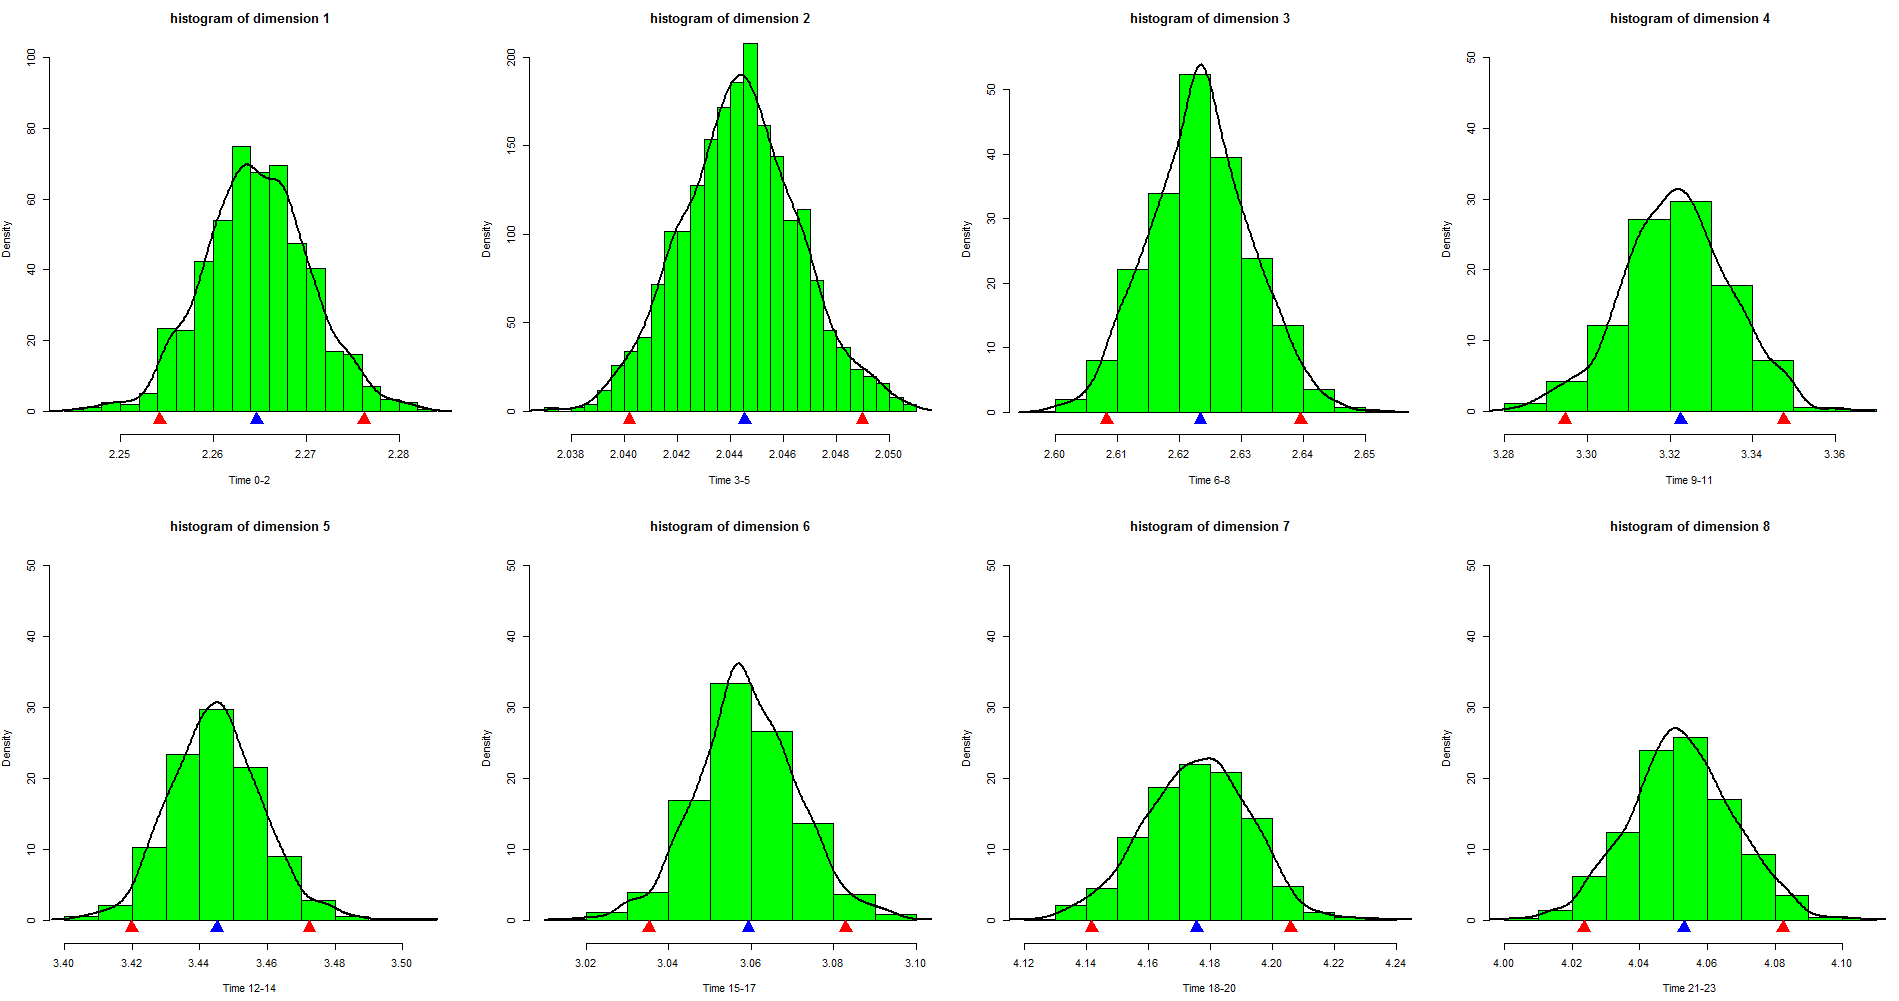
\epsfig{file=lm_data.PNG,angle=0, height=0.55\textwidth, width=0.9 \textwidth}
	\caption{Histograms of $B=1000$ perturbation-based SGD estimates for the POWER data. }
\end{figure}

\begin{figure}[htb]
	\centering
	\label{fig:fig-real-glm-1}
	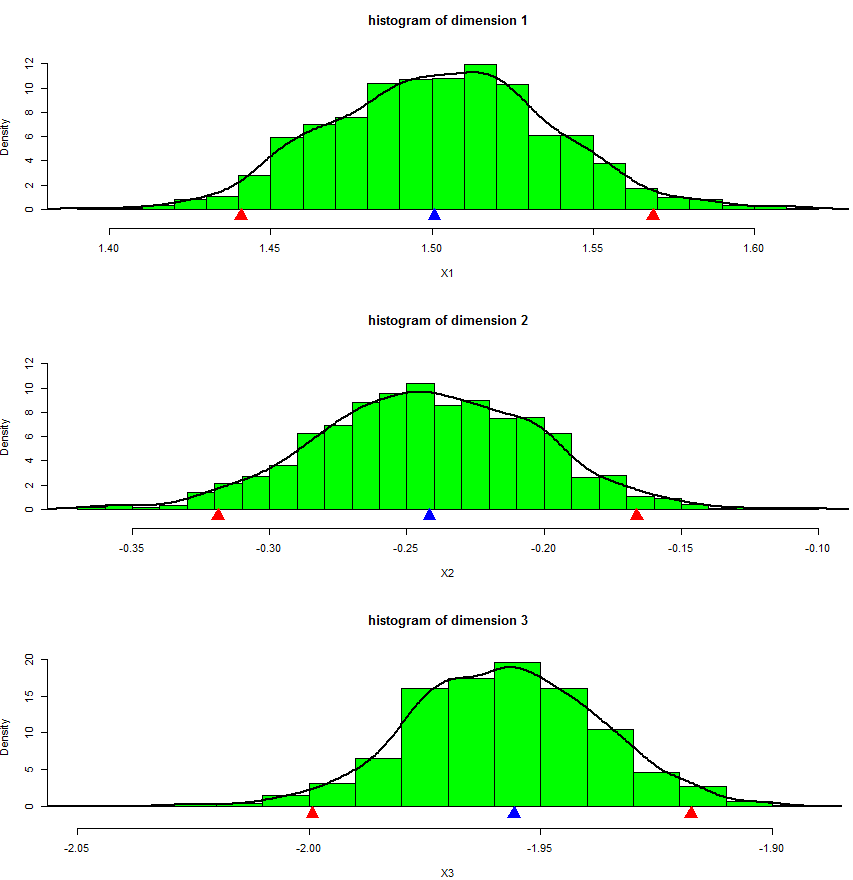
\epsfig{file=glm_data_1.PNG,angle=0, height=0.5\textwidth, width=0.5 \textwidth}
	\caption{Histograms of $B=1000$ perturbation-based SGD estimates for the SKIN data. }
\end{figure}

\begin{figure}[htb]
	\centering
	\label{fig:fig-real-glm-2}
	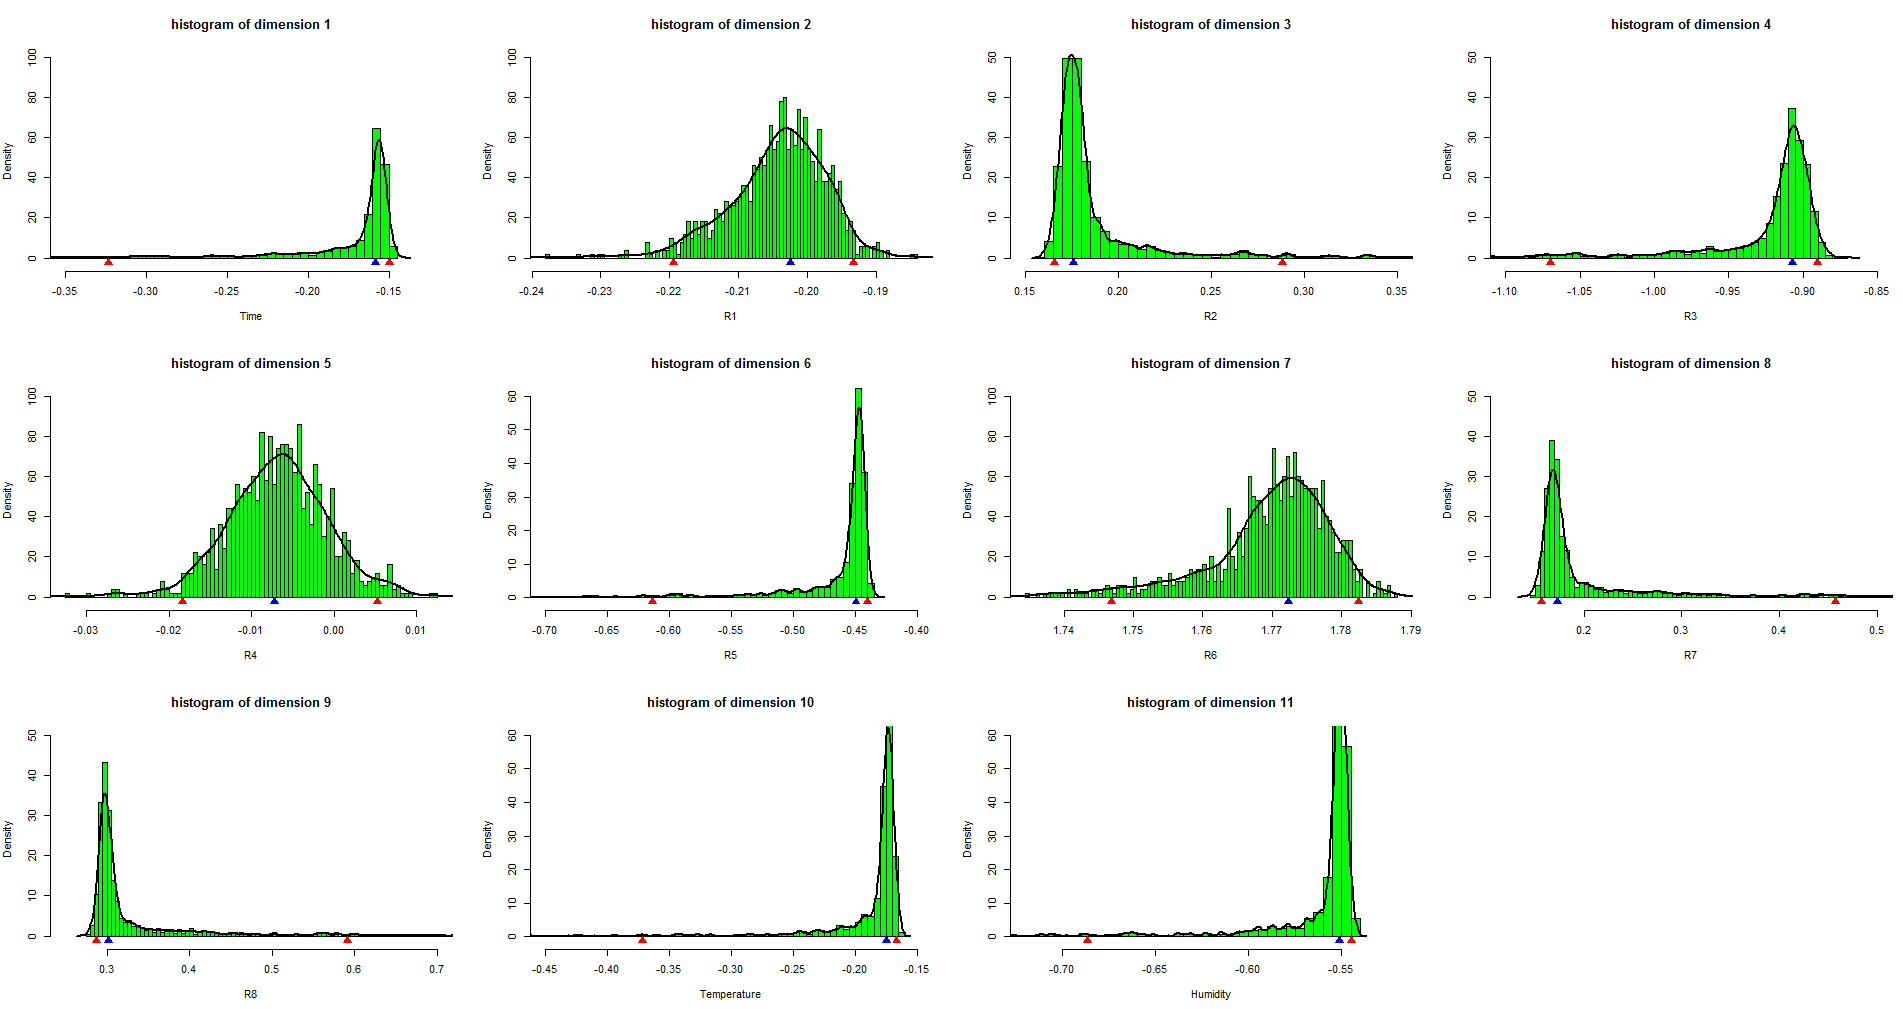
\epsfig{file=glm_data_2.PNG,angle=0, height=0.6\textwidth, width=0.9 \textwidth}
	\caption{Histograms of $B=1000$ perturbation-based SGD estimates for the GAS data. }
\end{figure}

\section{Discussion} \label{discussion}

Online updating is a useful strategy for analyzing big data and streaming data, and recently stochastic gradient decent has become a popular method for doing online updating. Although the asymptotic properties of SGD have been well studied, there is little research on conducting statistical inference based on SGD estimators. In this paper, we propose the perturbation-based resampling procedure, which can be applied to estimate the sampling distribution of an SGD estimator. The offline version of perturbation-based resamping procedure was first proposed by \citet{Rubin81} and was also discussed in \citet{Shao12}.

The proposed resampling procedure is in essence an online version of the bootstrap. Recall that the data points, $Z_1, Z_2, \dots, Z_N$, are arriving one at a time and an SGD estimate updates itself from $\wh{\theta}_{n-1}$ to $\wh{\theta}_n$ whenever a new data point $Z_n$ arrives. If we are forced to apply the bootstrap, then we should have many bootstrap samples; the data points of each bootstrap sample, $Z_1^*, Z_2^*, \dots, Z_N^*$, are assumed to be arriving one at a time and the bootstrapped SGD estimate updates itself from $\wh{\theta}^*_{n-1}$ to $\wh{\theta}^*_n$ whenever a new data point $Z_n^*$ arrives. Of course such bootstrap is impractical here because in online updating we will not obtain and store all the data points and then generate bootstrap samples. Now if we rearrange hypothetical bootstrap sample $Z_1^*, Z_2^*, \dots, Z_N^*$ as $\{K_1 {\rm \ copies\ } Z_1, K_2 {\rm \ copies\ } Z_2, \dots, K_N {\rm \ copies\ } Z_N\}$, where $K_n$ follows binomial distribution $B(N, 1/N)$, then the SGD estimator updates itself from $\wh{\theta}^*_{n-1}$ to $\wh{\theta}^*_n$ whenever a new batch of data points, $K_n$ copies of $Z_n$, arrives. Noting that binomial distribution $B(N, 1/N)$ approximates to Poisson distribution $P(1)$ as $N\rightarrow\infty$, we see that the aforementioned hypothetical bootstrap is equivalent to our proposed online bootstrap procedure with $W_n\sim P(1)$, whose mean and variance are both equal to one.

Finally, the SGD method considered in this paper is actually the explicit SGD, in contrast with the implicit SGD considered in \citet{Toulis17}. We are working on extending the proposed perturbation-based resampling procedure for conducting statistical inference for the implicit SGD.


\appendix
\section*{Appendix A. technical proofs}


For ease exposition of establishing
asymptotic normality of SGD and perturbed SGD estimates, we present the following Proposition 1, adapted from Theorem 2 of \citet[pp.841]{Polyak92}.
Let $R(\theta): \mathcal{R}^p \rightarrow \mathcal{R}^p$ be some unknown function and $R(\theta_0)=0$.
The dataset consists of $Z_n, n=1,2,\dots,$ which are i.i.d.~copies of $Z$. Stochastic
gradients are  $\wh{R}(\theta; Z_i)$ and $\mathbb{E}\{\wh{R}(\theta; Z_i)\}=R(\theta)$. With an initial point $\wh{\theta}_0$ and learning rates  $\gamma_n$, the SGD estimate is defined as
\begin{eqnarray}
\wh{\theta}_n=\wh{\theta}_{n-1} - \gamma_n \wh{R}(\wh{\theta}_{n-1}; Z_n)=\wh{\theta}_{n-1}-\gamma_n\left(R(\wh{\theta}_{n-1})-D_n\right),
\end{eqnarray}
where $D_n=R(\wh{\theta}_{n-1})-\wh{R}(\wh{\theta}_{n-1}; Z_n)$ is a martingale-difference process; that is, $\mathbb{E}\{D_n|\mathfrak{F}_{n-1}\}=0$, where $\mathfrak{F}_{n-1}=\sigma(\mathcal{D}_{n-1})$. The regularity conditions for Proposition 1 are
listed as follows.
\begin{enumerate}
	\item[(C1).] There exists a function $U(\theta): \mathcal{R}^p \rightarrow \mathcal{R}$ such that for some $\lambda>0$, $\delta>0$, $l_0>0$, $L_0>0$, and all $\theta, \theta'\in \mathcal{R}^p$, the conditions $U(\theta)\geq \lambda\|\theta\|^2$, $\|\nabla U(\theta) - \nabla U(\theta')\|\leq L_0\|\theta-\theta'\|$, $U(0)=0$, $\nabla U(\theta-\theta_0)\trans R(\theta)>0$ for $\theta\neq \theta_0$ hold true. Moreover, $\nabla U(\theta-\theta_0)\trans R(\theta)\geq \l_0 U(\theta-\theta_0)$ for all $\|\theta-\theta_0\|\leq \delta$.

	\item[(C2).] There exists a positive definite matrix $S_0\in \mathcal{R}^{p\times p}$ such that for some $C>0$, $0<\varrho\leq 1$, and $\delta>0$, the condition $\|R(\theta)-S_0(\theta-\theta_0)\| \leq C\|\theta-\theta_0\|^{1+\varrho}$ for all $\|\theta-\theta_0\|\leq \delta$ holds true.

	\item[(C3).] $\{D_n\}_{n\geq 1}$ is a martingale difference process with $\mathbb{E}\{D_n|\mathfrak{F}_{n-1}\}=0$, and for some $C>0$,
	$$\mathbb{E}\left\{\|D_n\|^2\left.\right|\mathfrak{F}_{n-1}\right\}+\|R(\wh{\theta}_{n-1})\|^2\leq C\left(1+\|\wh{\theta}_{n-1}\|^2\right)\mbox{\ a.s.,} $$
	for all $n\geq 1$. Consider decomposition $D_n=D_n(0)+E_n(\wh{\theta}_{n-1})$, where $D_n(0)=R(\theta_0)-\wh{R}(\theta_0; Z_n)$ and $E_n(\wh{\theta}_{n-1})=D_n-D_n(0)$. Assume that $\mathbb{E}\{D_n(0)|\mathfrak{F}_{n-1}\}=0$ a.s.,
	\begin{eqnarray*}
		&\mathbb{E}\{D_n(0)D_n(0)\trans|\mathfrak{F}_{n-1}\}\stackrel{P}{\rightarrow} V_0>0, \\
		&\sup_{n\geq 1}\mathbb{E}\left\{\|D_n(0)\|^2I(\|D_n(0)\|>\eta)|\mathfrak{F}_{n-1}\right\}\stackrel{P}{\rightarrow} 0, \mbox{\ as\ }\eta\rightarrow\infty,
	\end{eqnarray*}
	and there exists $\delta(x)\rightarrow 0$ as $x\rightarrow 0$ such that, for all $n$ large enough,
	$$\mathbb{E}\left\{\|E_n(\wh{\theta}_{n-1})\|^2\left.\right|\mathfrak{F}_{n-1}\right\}\leq \delta(\|\wh{\theta}_{n-1}-\theta_0\|) \mbox{\ \  a.s..}$$
	\item[(C4).] It holds that $(\gamma_n-\gamma_{n+1})/\gamma_n=o(\gamma_n)$, $\gamma_n>0$ for all $n$, and
	$\sum_{n=1}^{\infty}\gamma_n^{(1+\varrho)/2}n^{-1/2}<\infty.$
\end{enumerate}

Assumptions C2 and C4 are implied by the following Assumptions C2$'$ (i.e.~Assumption C2 with $\varrho=1$) and C4$'$ (i.e.~Assumption A5):
\begin{enumerate}
	\item[(C2$'$).] There exists a positive definite matrix $S\in \mathcal{R}^{p\times p}$ such that for some $C>0$ and $\delta>0$, the condition $\|R(\theta)-S_0(\theta-\theta_0)\| \leq C\|\theta-\theta_0\|^2$ for all $\|\theta-\theta_0\|\leq \delta$ holds true.
	\item[(C4$'$).] The learning rates are chosen as $\gamma_n=\gamma_1 n^{-\alpha}$ with $\gamma_1>0$ and $\alpha\in(0.5, 1)$.
\end{enumerate}


{\bf Proposition 1}. {\it If Assumptions C1-C4 are satisfied, then we have $\ol{\theta}_n\rightarrow\theta_0$,\ \ a.s.; and
	\begin{eqnarray}\label{sum-martingale-0}
	\sqrt{n}(\ol{\theta}_n-\theta_0)=\frac{1}{\sqrt{n}}S^{-1}\sum_{i=1}^n D_i+ o_p(1),
	\end{eqnarray}
	which implies $\sqrt{n}(\ol{\theta}_n-\theta_0) \Rightarrow \mathcal{N}\left(0, S_0^{-1}V_0S_0^{-1}\right), {\mbox \ in \ distribution.}$ }


\section*{A1. Proof of Lemma 1}

{\it Proof.} By Proposition 1, it suffices to show that Assumptions C1-C4 hold under Assumptions A1-A5. Because C2 and C4 are implied by C2$'$ and C4$'$, it suffices to show that Assumptions C1, C2$'$, C3 and C4$'$ hold under Assumptions A1-A5.

{\it Verification of Assumption C1:} Recall that $R(\theta)=\nabla L(\theta)$ and $\wh{R}(\theta; Z_i)=\nabla \ell(\theta; Z_i)$. Define $U(\theta)=L(\theta_0+\theta)-L(\theta_0)+\lambda\|\theta\|^2$ for a given $\lambda>0$. By definition of $U(\theta)$ and Assumption A1, we have $U(\theta)\geq \lambda \|\theta\|^2$ and $U(0)=0$. For any $\theta$ and $\theta'$, since $\nabla U(\theta)-\nabla U(\theta')=R(\theta+\theta_0)-R(\theta'+\theta_0)+2\lambda(\theta-\theta')$, letting $L_0=L_1+2\lambda$ and by Assumption A2, we have $\|\nabla U(\theta)-\nabla U(\theta')\|\leq L_1\|\theta-\theta'\|$. Since $\nabla U(\theta-\theta_0)\trans R(\theta)=\|R(\theta)\|^2+\lambda (\theta-\theta_0)\trans R(\theta)$, by Assumption A1, we have $\nabla U(\theta-\theta_0)\trans R(\theta)>0$ for any $\theta\neq \theta_0$. Last, it remains to verify there exist $l_0>0$ and $\delta>0$ such that $\nabla U(\theta-\theta_0)\trans R(\theta)\geq \l_0 U(\theta-\theta_0)$ for all $\|\theta-\theta_0\|\leq \delta$. Noting that $U(\theta-\theta_0)=L(\theta+\theta_0)+\lambda\|\theta-\theta_0\|^2$, by Taylor expansion and Assumption A3, we see that there exist $l_1>0$ and $\delta_1$ such that $U(\theta-\theta_0)\leq l_1 \|\theta-\theta_0\|^2$ for all $\|\theta-\theta_0\|\leq \delta_1$. On the other hand, noting that $\nabla U(\theta-\theta_0)\trans R(\theta)=\|R(\theta)\|^2 + \lambda(\theta-\theta_0)\trans R(\theta)$, by Assumption A3 also, we see that there exist $l_2>0$ and $\delta_2$ such that $(\theta-\theta_0)\trans R(\theta)\geq l_2 \|\theta-\theta_0\|^2$ for all $\|\theta-\theta_0\|\leq \delta_2$. Selecting $\delta=\min(\delta_1, \delta_2)$ and $l_0=\lambda l_2/l_2$, we show that $\nabla U(\theta-\theta_0)\trans R(\theta)\geq \l_0 U(\theta-\theta_0)$ for all $\|\theta-\theta_0\|\leq \delta$.

{\it Verification of Assumption C2$'$:} Recall that $R(\theta)=\nabla L(\theta)$, $S(\theta)=\nabla R(\theta)$, and $S_0=S(\theta_0)>0$. By Assumption A3, there exists $\delta>0$ such that for any $\|\theta-\theta_0\|<\delta'$, $\|S(\theta)-S(\theta_0)\|<L_2\|\theta-\theta_0\|$. By mean-value theorem, $\|S(\theta)-S_0(\theta-\theta_0)\|=\|S(\wt{\theta})(\theta-\theta_0)-S_0(\theta-\theta_0)\|$, where $\wt{\theta}$ lies between $\theta$ and $\theta_0$. Hence $\|S(\theta)-S_0(\theta-\theta_0)\|\leq L_2\|\theta-\theta_0\|^2$, for any $\|\theta-\theta_0\|\leq \delta$. Letting $C=L_2$, we have verified Assumption C2$'$.

{\it Verification of Assumption C3:}  $D_n=R(\wh{\theta}_{n-1})-\wh{R}(\wh{\theta}_{n-1}; Z_n)$. Consider decomposition $D_n=D_n(0)+E_n(\wh{\theta}_{n-1})$, where $D_n(0)=-\nabla \ell(\theta_0, Z_n)$ and $E_n(\wh{\theta}_{n-1})=[R(\wh{\theta}_{n-1})-R(\theta_0)]-[\nabla \ell(\wh{\theta}_{n-1}; Z_n)-\nabla \ell(\theta_0; Z_n)]$. By Assumption A2, $\|R(\wh{\theta}_{n-1})\|^2\leq L_1^2 \|\wh{\theta}_{n-1}-\theta_0\|^2$. In addition, Cauchy-Schwartz inequality implies that $\mathbb{E}\left\{\|\nabla \ell(\theta; Z_n)-\nabla \ell(\theta_0; Z_n)\|^2\right\}=2\mathbb{E}\|\nabla \ell(\theta; Z_n)\|^2+2\mathbb{E}\|\nabla \ell(\theta_0; Z_n)\|^2$; we have $\mathbb{E}\left\{\|\nabla \ell(\wh{\theta}_{n-1}; Z_n)-\nabla \ell(\theta_0; Z_n)\|^2\left.\right|\right\}\leq C'(1+\|\theta\|^2)$ for some $C'>0$ by Assumption A4, . Together, we have  $\mathbb{E}\left\{\|D_n\|^2\left.\right|\mathfrak{F}_{n-1}\right\}+\|R(\wh{\theta}_{n-1})\|^2\leq C\left(1+\|\wh{\theta}_{n-1}\|^2\right)$ for some $C>0$. Moreover, because $D_n(0)$'s are i.i.d., we have $\mathbb{E}\{D_n(0)D_n(0)\trans|\mathfrak{F}_{n-1}\}=V_0>0$ and
$\sup_{n\geq 1}\mathbb{E}\left\{\|D_n(0)\|^2I(\|D_n(0)\|>\eta)|\mathfrak{F}_{n-1}\right\}\stackrel{P}{\rightarrow} 0$, as $\eta\rightarrow\infty$. Finally, note that $\mathbb{E}\|E_n(\theta)\|^2\leq L^2_1\|\theta-\theta_0\|^2+\mathbb{E}\|\nabla \ell(\theta; Z_n)-\nabla \ell(\theta_0; Z_n)\|^2$. By Assumption A3, $\mathbb{E}\|\nabla \ell(\theta; Z_n)-\nabla \ell(\theta_0; Z_n)\|^2\leq \delta'(\|\theta-\theta_0\|)$ for some $\delta'(\cdot)$ with $\delta'(x)\rightarrow 0$ as $x\rightarrow 0$. Define $\delta(x)=L_1^2 x^2 + \delta'(x)$, we show $\mathbb{E}\|E_n(\theta)\|^2\leq \delta(\|\theta-\theta_0\|)$. This complete the verification of Assumption C3.

Obviously Assumption A5 is the same as Assumption C4$'$. Therefore, we have verified that Assumptions A1-A5 imply Assumptions C1, C2$'$, C3 and C4$'$. By Proposition 1, we complete the proof of Lemma 1. $\Box$


\section*{A2. Proof of Theorem 1}

{\it Proof.} Rewrite $\wh{\theta}^*_n$ as
\begin{eqnarray}\label{SGD-wt-rewrite}
\wh{\theta}^*_n = \wh{\theta}^*_{n-1}-\gamma_n R(\wh{\theta}^*_{n-1})+\gamma_n D^*_n,\label{SGD-wt-rewrite}
\end{eqnarray}
where $D^*_n=R(\wh{\theta}^*_{n-1})-W_n\nabla \ell(\wh{\theta}^*_{n-1}; Z_n)$. Then let $\mathfrak{F}^*_{n-1}$ be the Borel field generated by $\{(Z_i, W_i), i\leq n-1\}$.
Since $\mathbb{E}\{W_n|\mathfrak{F}^*_{n-1}\}=1$ and $R(\theta)=\mathbb{E}\{\nabla \ell(\theta; Z_n)\}$, we have $\mathbb{E}\{D^*_n|\mathfrak{F}_{n-1}\}=0$. Thus $D^*_n$ is a martingale-difference process.
Let $D^*_n(\theta)=R(\theta)-W_n\nabla \ell(\theta; Z_n)$. Consider decomposition $D^*_n=D^*_n(0)+E^*_n(\wh{\theta}^*_{n-1})$, where
\begin{eqnarray}
D^*_n(0)=-W_n\nabla \ell(\theta_0; Z_n)
\end{eqnarray}  and
\begin{equation}
E^*_n(\theta)=[R(\theta)-R(\theta_0)]-W_n[\nabla \ell(\theta; Z_n)-\nabla \ell(\theta_0; Z_n)].
\end{equation}
Noting that $\mathbb{E}\{D^*_n(0)\}=0$ and $\mathbb{E}(W_n^2)=2$ under Assumption A6, by Assumption A4, we have
\begin{equation}\label{D-0}
\mathbb{E}\{[D^*_n(0)][D^*_n(0)]\trans\}=2\mathbb{E}\left\{[\ell(\theta_0; Z_n)][\ell(\theta_0; Z_n)]\trans\right\}=2V_0.
\end{equation}
By Cauchy-Schwartz inequality and Assumptions A2 and A4, we have
\begin{equation}\label{E-n}
\mathbb{E}\{\|E_n^*(\theta)\|^2\}\leq 2\|R(\theta)\|^2 + 4\mathbb{E}\left\{\|\nabla \ell(\theta, Z)-\nabla \ell(\theta_0, Z)\|^2\right\}\leq \delta'(\|\theta-\theta_0\|),
\end{equation}
where $\delta'(x)= 2L_1^2x^2+2\delta(x)$ satisfying that $\delta'(x)\rightarrow 0$ as $x\rightarrow 0$. Also by Cauchy-Schwartz inequality, $\mathbb{E}\{\|E^*_n(\theta)\|^2\}\leq 2\|R(\theta)\|^2+2\mathbb{E}\{\|\nabla \ell(\theta, Z)\|^2\}$. Further, by Assumptions A2 and A4,
\begin{equation}\label{D-n}
\mathbb{E}\{\|D_n^*\|^2|\mathfrak{F}_{n-1}\}+\|R(\wh{\theta}^*_{n-1})\|^2\leq 3L_1^2\|\wh{\theta}^*_{n-1}-\theta_0\|^2 + 2C\|\wh{\theta}^*_{n-1}\|^2\leq C' (1+\|\wh{\theta}^*_{n-1}-\theta_0\|^2),
\end{equation}
for some large enough $C'>0$. Combining results (\ref{D-0})-(\ref{D-n}), we have verified Assumption C3. Moreover, noting that $\mathbb{E}W_n=1$, we can easily verify that Assumptions A1 and A2 imply that Assumption C1 holds, and Assumption A3 implies that Assumption C2 holds. By Proposition 1, we show that $\wh{\theta}^*_n\rightarrow\theta_0$ almost surely, and
\begin{eqnarray}\label{sum-martingale}
\sqrt{n}(\ol{\theta}_n^*-\theta_0)&=&\frac{1}{\sqrt{n}}S_0^{-1}\sum_{i=1}^n D_i^*+ o_p(1)\nonumber\\
&=& -\frac{1}{\sqrt{n}}S_0^{-1}\sum_{i=1}^n W_i \nabla \ell(\theta_0; Z_i)+\frac{1}{\sqrt{n}}S_0^{-1}\sum_{i=1}^n E^*_n(\wh{\theta}^*_{n-1})+o_p(1).
\end{eqnarray}
Note that $\mathbb{E}\{\|E_n(\wh{\theta}^*_{n-1})\|^2|\mathfrak{F}_{n-1}\}\leq \delta'(\|\wh{\theta}^*_{n-1}-\theta_0\|)$, following (\ref{E-n}). Since $\wh{\theta}^*_n\rightarrow\theta_0$ a.s., we have $\delta(\|\wh{\theta}^*_{n-1}-\theta_0\|)\rightarrow 0$ a.s.. Thus, $S_0^{-1}\sum_{i=1}^n E_n(\wh{\theta}^*_{n-1})/\sqrt{n}=o_p(1)$. Therefore, by (\ref{sum-martingale}), this completes the proof of Theorem 1. $\Box$

\section*{A3. Proof of Theorem 2}

{\it Proof.}  Let
\begin{equation}\label{V-n}
V_n=-\frac{1}{\sqrt{n}}S_0^{-1}(W_i-1)\nabla \ell(\theta_0, Z_i).
\end{equation}
By Theorem 1, we have $\sqrt{n}(\ol{\theta}^*_n-\ol{\theta}_n)=V_n+o_p(1)$. We first show that, for any $\beta \in \mathbf{B}\triangleq\{\beta\in\mathcal{R}^p: \|\beta\|=1\}$ and $u\in\mathcal{R}$,
\begin{equation}\label{CLT-alpha}
\mathbb{P}^*\left(\beta\trans V_n\leq u\right)\rightarrow\Phi(u/\sigma_{\beta}), {\mbox{\ in\ probability}},
\end{equation}
where $\Phi(u)$ is the distribution of $\mathcal{N}(0, 1)$ and $\sigma_{\beta}=\beta\trans S_0^{-1}V_0 S_0^{-1}\beta$. In fact,
\begin{equation}\label{V-n-xi}
\beta\trans V_n=\frac{1}{\sqrt{n}} \sum_{i=1}^n (W_i-1)\xi_i,
\end{equation}
where $\xi_i=-\beta\trans S_0^{-1}\nabla \ell(\theta_0, Z_i)$. Note that, by Assumption A6, $\mathbb{E} W_i= \Var(W_i)=1$. Hence
\begin{equation}\label{s-n}
s_n=\frac{1}{n}\sum_{i=1}^n{\Var}^*\{(W_i-1)\xi_i\}=\frac{1}{n}\sum_{i=1}^n\xi_i^2\rightarrow \sigma^2_{\beta}, {\mbox{\ in\ probability}},
\end{equation}
and for any $\epsilon>0$,
\begin{equation}\label{Lind-cond}
\frac{1}{ns_n}\sum_{i=1}^{n}\mathbb{E}^*\left\{(W_i-1)^2\xi_i^2I\left[|(W_i-1)\xi_i|>\sqrt{n}s_n\epsilon\right]\right\}\rightarrow 0, {\mbox{\ in\ probability}}.
\end{equation}
Therefore, the Lindeberg's condition is satisfied. By the central limit theorem, (\ref{CLT-alpha}) holds, which implies that for any $\beta \in \mathbf{B}$,
\begin{equation}\label{CLT-alpha-sup}
\sup_{u\in\mathcal{R}}\left|\mathbb{P}^*\left(\beta\trans V_n\leq u\right)-\Phi(u/\sigma_{\beta})\right|\rightarrow 0, {\mbox{\ in\ probability}}.
\end{equation}
Consider $\mathbf{B}_0\triangleq\{\beta\in\mathcal{R}^p: \|\beta\|=1, \mbox{the\ components\ of\ }\beta \mbox{\ are\ rational}\}$, which contains only countable many $\beta$ and is a dense subset of $\mathbf{B}$. For any subsequence $\{n_1\}$, by Cantor's ``diagonal method" used in \citet{Rao92}, we can show that there exists a subsequence $\{n_2\}\subset \{n_1\}$ such that, with probability one,
\begin{equation}\label{CLT-alpha-sup-any}
\sup_{u\in\mathcal{R}}\left|\mathbb{P}^*\left(\beta\trans V_{n-1}\leq u\right)-\Phi(u/\sigma_{\beta})\right|\rightarrow 0, \mbox{\ for \ any \ } \beta\in\mathbf{B}_0.
\end{equation}
Hence, we show that
\begin{equation}\label{eq-co-1}
\sup_{v\in\mathcal{R}^p}\left|\mathbb{P}^*\left(\sqrt{n}(\ol{\theta}^*_n-\ol{\theta}_n)\leq v\right)-\mathbb{P}(\zeta\leq v)\right| \rightarrow 0, {\mbox{\ in\ probability}},
\end{equation}
where $\zeta\sim\mathcal{N}(0, S_0^{-1}V_0S_0^{-1})$. By Lemma 1, we can also show that
\begin{equation}\label{eq-co-2}
\sup_{v\in\mathcal{R}^p}\left|\mathbb{P}\left(\sqrt{n}(\ol{\theta}_n-\theta_0)\leq v\right)-\mathbb{P}(\zeta\leq v)\right| \rightarrow 0.
\end{equation}
Combining (\ref{eq-co-1}) and (\ref{eq-co-2}), we complete the proof of Theorem 2. $\Box$\\

\section*{A4. Proof of Lemma 2}

{\it Proof.} By Proposition 1, it suffices to show that Assumptions C1, C2$'$ and C3 hold under Assumptions B1-B4.

{\it Verification of Assumption C1:} Define $\Delta=\theta-\theta_0$. Let $R(\Delta)=\mathbb{E}\{\phi(\Delta\trans X|X)X\}$ and $\wh{R}(\Delta; Z_n)=\psi(\Delta\trans X_n+\varepsilon_n)X_n$. Define $U(\Delta)=\Delta\trans\Delta$. By definition of $U(\Delta)$, $U(\Delta)\geq \lambda \|\Delta\|^2$ with $\lambda=1$, $U(0)=0$ and $\nabla U(\Delta)$ is Lipschitz continuous. Since $\Delta\trans\mathbb{E}\{\phi(\Delta\trans X|X)\Delta\trans X\}>0$ by Assumption B3, we see that $\nabla U(\Delta)\trans R(\Delta)>0$. By the mean-value theorem and by Assumption B3, there exists $\delta$ such that $\Delta\trans\mathbb{E}\{\phi(\Delta\trans X|X)\Delta\trans X\}\geq\Delta\trans\mathbb{E}\{\dot{\phi}(0|X) XX\trans\}\Delta/2\geq \lambda_{\min}(S_0)\|\Delta\|^2/2$, for any $\|\Delta\|\leq \delta$, where $\lambda_{\min}(S_0)$ is the minimum eigenvalue of $S_0$. Hence $\nabla U(\Delta)\trans R(\Delta)\geq \lambda_{\min}(S_0)\|\Delta\|^2$ and we have verified Assumption C1.


{\it Verification of Assumption C2$'$:} Note that $$
\|R(\Delta)-S_0\Delta\|=\|\mathbb{E}\phi(\Delta\trans X|X)-\mathbb{E}\dot{\phi}(0|X)XX\trans\Delta\|.$$ By the mean-value theorem and Assumption B4, there exists $\delta$ such that, for any $\|\Delta\|\leq \delta$, $\|\mathbb{E}\{\phi(\Delta\trans X|X)X\}-\mathbb{E}\{\dot{\phi}(0|X)XX\trans\Delta\}\|\leq C_2\lambda_{\max}(S_0)\|\Delta\|^2$. This implies Assumption C2$'$.

{\it Verification of Assumption C3:}  Let $\wh{\Delta}_{n}=\wh{\theta}_{n}-\theta_0$. Then $D_n=R(\wh{\Delta}_{n-1})-\wh{R}(\wh{\Delta}_{n-1}; Z_n)$. Consider decomposition $D_n=D_n(0)+E_n(\wh{\Delta}_{n-1})$, where $D_n(0)=\psi(\varepsilon_n)X_n$ and $E_n(\wh{\Delta}_{n-1})=\mathbb{E}\{\psi(\wh{\Delta}_{n-1}\trans X+\varepsilon_n)X_n\}-[\psi(\wh{\Delta}_{n-1}\trans X+\varepsilon_n)X_n -\psi(\varepsilon_n)X_n]$. By Assumption B1 and the Cauchy-Schwartz inequality, we can show that  $\mathbb{E}\left\{\|D_n\|^2\left.\right|\mathfrak{F}_{n-1}\right\}+\|R(\wh{\Delta}_{n-1})\|^2\leq 2C_1\left(1+\|\wh{\Delta}_{n-1}\|^2\right)$. Moreover, by Assumption B2, $D_n(0)$'s are i.i.d., so $\mathbb{E}\{D_n(0)D_n(0)\trans|\mathfrak{F}_{n-1}\}=V_0>0$ and
$\sup_{n\geq 1}\mathbb{E}\left\{\|D_n(0)\|^2I(\|D_n(0)\|>\eta)|\mathfrak{F}_{n-1}\right\}{\rightarrow} 0$, as $\eta\rightarrow\infty$. Finally, by Cauchy-Schwartz inequality and Assumptions B2-B3, we can show that $\mathbb{E}\|E_n(\Delta)\|^2\leq \delta(\|\Delta\|)$ for some $\delta(\cdot)$ with $\delta(x)\rightarrow 0$ as $x\rightarrow 0$. This complete the verification of Assumption C3.

Obviously Assumption A5 is the same as Assumption C4$'$. Therefore, we have verified that Assumptions B1-B4 and A5 imply Assumptions C1, C2$'$, C3 and C4$'$. By Proposition 1, we complete the proof of Lemma 2. $\Box$

\section*{A5. Proof of Theorem 3}

{\it Proof.} Recall that $R(\Delta)=\mathbb{E}\{\phi(\Delta\trans X|X)X\}$ and $\wh{\Delta}_{n}=\wh{\theta}_{n}-\theta_0$. Rewrite $\wh{\theta}^*_n$ as
\begin{eqnarray}\label{SGD-wt-rewrite}
\wh{\theta}^*_n = \wh{\theta}^*_{n-1}+\gamma_n R(\wh{\Delta}_{n})+\gamma_n D^*_n,\label{SGD-M-wt-rewrite}
\end{eqnarray}
where $D^*_n=W_n\psi(\wh{\Delta}_{n}\trans X_n + \varepsilon_n)X_n-R(\wh{\Delta}_{n})$ is a martingale-difference process
by Assumption B3 and that $\mathbb{E}\{W_n|\mathfrak{F}_{n-1}\}=1$.
Let $D^*_n(\Delta)=W_n\psi\left(\Delta\trans X_n + \varepsilon_n\right)X_n-R(\Delta)$ and $D^*_n(\Delta)=D^*_n(0)+E^*_n(\Delta)$, where
\begin{equation}
E^*_n(\Delta)=W_n\left[\psi(\Delta\trans X_n+\varepsilon_n)-\psi(\varepsilon_n)\right]X_n-R(\Delta).
\end{equation}
Since $D^*_n(0)=W_n\psi(\varepsilon_n)X_n$, $\mathbb{E}\{D^*_n(0)\}=0$ and $\mathbb{E}\{[D^*_n(0)][D^*_n(0)]\trans\}=(1+\Var(W_1))V_0$ by Assumption B2. By Cauchy-Schwartz inequality and Assumptions B2-B3, we can show that $\mathbb{E}\|E^*_n(\Delta)\|^2\leq \delta(\|\Delta\|)$ for some $\delta(\cdot)$ with $\delta(x)\rightarrow 0$ as $x\rightarrow 0$.  Therefore, using the similar arguments as those in the proof of Lemma 2, we can verify that, under Assumptions B1-B4, Assumptions  C1-C4 are satisfied. By Proposition 1, it follows that $\wh{\theta}^*_n\rightarrow\theta_0$ almost surely, and
\begin{eqnarray}\label{sum-M-martingale}
\sqrt{n}(\ol{\theta}_n^*-\theta_0)=\frac{1}{\sqrt{n}}S_0^{-1}\sum_{i=1}^n D_i^*+ o_p(1).
\end{eqnarray}
By the decomposition of $D_i^*$, we have
\begin{eqnarray}\label{sum-M-martingale-decom}
\sqrt{n}(\ol{\theta}_n^*-\theta_0)=\frac{1}{\sqrt{n}}S_0^{-1}\sum_{i=1}^n W_i \psi(\varepsilon_i)X_i+\frac{1}{\sqrt{n}}S_0^{-1}\sum_{i=1}^n E^*_n(\wh{\theta}^*_{n-1}-\theta_0)+o_p(1).
\end{eqnarray}
By the definition of $\delta(\|\Delta\|)$,  $\mathbb{E}\{\|E^*_n(\wh{\theta}^*_{n-1}-\Delta)\|_2^2|\mathfrak{F}_{n-1}\}=\delta(\|\wh{\theta}^*_{n-1}-\theta_0\|)$.
Since $\wh{\theta}^*_n\rightarrow\theta_0$ a.s., we have $\delta(\|\wh{\theta}^*_{n-1}-\theta_0\|)\rightarrow 0$ a.s.. Thus, $\sum_{i=1}^n E^*_n(\wh{\theta}^*_{n-1}-\theta_0)/\sqrt{n}=o_p(1)$. By (\ref{sum-M-martingale-decom}), we complete the proof of Theorem 3. $\Box$

\vskip 0.2in
\begin{thebibliography}{99}
\bibitem[Moulines and Bach(2011)]{Moulines11} {Moulines, Eric and Bach, Francis R}. Non-asymptotic analysis of stochastic approximation algorithms for machine learning. {\it Advances in Neural Information Processing Systems}, 451--459, 2011.

\bibitem[Chen et al.(2016)]{Chen16} {Chen, Xi and Lee, Jason D and Tong, Xin T and Zhang, Yichen}. Statistical Inference for Model Parameters in Stochastic Gradient Descent. {\it arXiv preprint arXiv:1610.08637}, 2016.

\bibitem[Efron(1979)]{Efron79} {Efron, Bradley}. Bootstrap methods: Another look at the jackknife. {\it Annals of Statistics}, {7}, 1-26.

\bibitem[Wang et al.(2016)]{Wang16} {Wang, Chun and Chen, Ming-Hui and Schifano, Elizabeth and Wu, Jing and Yan, Jun}. Statistical methods and computing for big data. {\it Statistics and its interface}, {9}, 399.

\bibitem[Hastie et al.(2009)]{Hastie09} {Hastie, Trevor and Tibshirani, Robert and Friedman, Jerome}. The elements of statistical learning 2nd edition. {\it New York: Springer}, 2009.

\bibitem[Kushner and Yin(2003)]{Kushner03} {Kushner, Harold and Yin, G George}. Stochastic approximation and recursive algorithms and applications. {\it Springer Science \& Business Media}, 2003.

\bibitem[Li et al.(2017)]{Li17} {Li, Tianyang and Liu, Liu and Kyrillidis, Anastasios and Caramanis, Constantine}. Statistical methods and computing for big data. {\it arXiv preprint arXiv:1705.07477}, 2017.

\bibitem[Nelder and Baker(1972)]{Nelder72} {Nelder, John A and Baker, R Jacob}. Generalized linear models. {\it Encyclopedia of statistical sciences}, 1972.

\bibitem[Polyak and Juditsky(1992)]{Polyak92} {Polyak, Boris T and Juditsky, Anatoli B}. Acceleration of stochastic approximation by averaging. {\it SIAM Journal on Control and Optimization}, {30}, 838--855.

\bibitem[Rao and Zhao(1992)]{Rao92} {Rao, C Radhakrishna and Zhao, LC}. Approximation to the distribution of M-estimates in linear models by randomly weighted bootstrap. {\it Sankhy{\=a}: The Indian Journal of Statistics, Series A}, 323--331.

\bibitem[Robbins and Monro(1951)]{Robbins51} {Robbins, Herbert and Monro, Sutton}. A stochastic approximation method. {\it The annals of mathematical statistics}, 400--407.

\bibitem[Rubin(1981)]{Rubin81} {Rubin, Donald B}. The bayesian bootstrap. {\it The annals of statistics}, {9}, 130--134.

\bibitem[Ruppert(1988)]{Ruppert88} {Ruppert, David}. Efficient estimations from a slowly convergent Robbins-Monro process. {\it Cornell University Operations Research and Industrial Engineering}, 1988.

\bibitem[Shao and Tu(2012)]{Shao12} {Shao, Jun and Tu, Dongsheng}. The jackknife and bootstrap. {\it Springer Science \& Business Media}, 2012.

\bibitem[Su and Zhu(2018)]{Su18} {Su, Weijie and Zhu, Yuancheng}. Statistical Inference for Online Learning and Stochastic Approximation via Hierarchical Incremental Gradient Descent. {\it arXiv preprint arXiv:1802.04876}, 2018.

\bibitem[Toulis et al(2017)]{Toulis17} {Toulis, Panos and Airoldi, Edoardo M and others}. Asymptotic and finite-sample properties of estimators based on stochastic gradients. {\it The Annals of Statistics}, {45}, 1694--1727.


\end{thebibliography}

\end{document}
